% \documentclass{article} % article 文档

% \usepackage[UTF8]{ctex}  % 使用宏包(为了能够显示汉字)
\documentclass[UTF8]{ctexart}
% \usepackage{geometry}
% \geometry{left=3.18cm,right=3.18cm,top=2.54cm,bottom=2.54cm}
\usepackage{graphicx}
\pagestyle{plain}    
\usepackage{setspace}
\usepackage{array}
\usepackage{booktabs} %调整表格线与上下内容的间隔
\usepackage{multirow}

\usepackage[a4paper]{geometry}
\usepackage{amsmath}

\usepackage{authblk}
\usepackage{longtable}
\usepackage{tabularx}
\usepackage{graphicx} 
\usepackage{subfigure}
\usepackage{float}
\usepackage{pifont}

\usepackage{listings}
\usepackage{xcolor} 
\definecolor{mygreen}{rgb}{0,0.6,0}
\definecolor{mygray}{rgb}{0.5,0.5,0.5}
\definecolor{mymauve}{rgb}{0.58,0,0.82}
\lstset{ %
backgroundcolor=\color{white},   % choose the background color
basicstyle=\footnotesize\ttfamily,        % size of fonts used for the code
columns=fullflexible,
breaklines=true,                 % automatic line breaking only at whitespace
captionpos=b,                    % sets the caption-position to bottom
tabsize=4,
commentstyle=\color{mygreen},    % comment style
escapeinside={\%*}{*)},          % if you want to add LaTeX within your code
keywordstyle=\color{blue},       % keyword style
stringstyle=\color{mymauve}\ttfamily,     % string literal style
frame=shadowbox,
rulesepcolor=\color{red!20!green!20!blue!20},
% identifierstyle=\color{red},
numbers=left, 
numberstyle=\tiny,
% escapeinside=' ',
xleftmargin=2em,
xrightmargin=2em, 
aboveskip=1em
}

\usepackage{hyperref}
\hypersetup{hypertex=true,
colorlinks=true,
linkcolor=blue,
anchorcolor=blue,
citecolor=blue}


\date{}
\begin{document}
\pagestyle{empty}

\includegraphics[]{guangdong.jpg}%学校图标
\begin{center}
    
\includegraphics[scale=0.5]{gdut.jpg}%学校图标
\end{center}
\begin{center}
	\quad \\
	\heiti \fontsize{22}{18} \textbf{《Python数值分析》}
    \vskip 1.0cm
\end{center}
\begin{center}
	\heiti \fontsize{22}{18} \textbf{课程报告}
	\vskip 2.5cm
\end{center}
\begin{center}
	\begin{tabular}{l}
		
		学~~~~~~院 \underline{~~~~~~~~计算机学院~~~~~~~~~~~~~~~~~}\\\\
		专~~~~~~业 \underline{~~~~~~~~计算机科学与技术~~~~~~~~~~}\\\\
		% \quad 代表空格,输入题目后自己调长度
		班~~~~~~级 \underline{~~~~~~~~4班~~~~~~~~~~~~~~~~~~~~~~~~~}\\\\
    学~~~~~~号 \underline{~~~~~~~~3120005057~~~~~~~~~~~~~~~~~~}\\\\
    学生姓名 \underline{~~~~~~~~陈嘉浩~~~~~~~~~~~~~~~~~~~~~~~~~}\\\\
		授课教师 \underline{~~~~~~~~龚怡~~~~~~~~~~~~~~~~~~~~~~~~~~~}\\\\

	\end{tabular}
\end{center}
\begin{center}
        \vskip 1cm
		{2022} 年{\quad 05}月
		
\end{center}
\newpage


% 生成目录设置
\begin{center}
  \renewcommand{\contentsname}{目录} %将content转为目录
\end{center}
\begin{center}
  \tableofcontents
\end{center}
\setcounter{page}{0}
\thispagestyle{empty} 
\newpage

\section{绪论}
\subsection{数值分析的发展综述}
早在在三十年前, 计算数学的先驱之一 L. N. Trefethen 就给出了数值分析的定义:

Numerical~ analysis is the study of algorithms for the problems of continuous problems.

---Lloyd N. Trefethen, Cornell University

翻译过来就是: 数值分析是研究连续问题的算法的科学. 其中, 最主要的概念就是算法和连续问题. 首先, 连续问题是从物理或者其它学科中抽象出来的复杂模型问题, 一般是无穷维问题且几乎无法找到解析解. 这些棘手的连续问题就自然成为数值分析的目标对象. 其次, 求解连续问题的算法的设计和分析是数值分析的核心内容, 它们的目的是将连续的无穷维的问题离散化, 得到一个离散的有限维的可解问题, 进而得到近似解. 如果没有数值分析, 现代科学与工程应用研究将很快陷入停滞.

数值分析领域比现代计算机的发明早了好几个世纪。线性插值在 2000 多年前就已经在使用。
过去许多伟大的数学家都专注于数值分析,从牛顿法、拉格朗日插值多项式、高斯消元法或欧拉法等重要算法的名称中可以明显看出这一点。

为方便手工计算,制作了带有插值点和函数系数等公式和数据表的大型书籍。
使用这些表格,对于某些函数,通常计算到小数点后 16 位或更多,人们可以查找值以插入给定的公式并获得对某些函数的非常好的数值估计。
该领域的权威著作是由Abramowitz和Stegun编辑的NIST出版物,这本1000多页的书中包含了大量常用的公式和函数,
以及它们在许多点上的值。当有计算机可用时,函数值不再很有用,但大量的公式列表仍然非常方便。

机械计算器也被开发为手动计算的工具。这些计算器在 1940 年代演变成电子计算机,然后发现这些计算机也可用于管理目的。
但是计算机的发明也影响了数值分析领域,因为现在可以进行更长更复杂的计算。

当今的主要研究领域有:1.函数求值;2.内插法、外推法、曲线拟合及回归;3.求解方程及方程组;4.求解特征值或奇异值问题
;5.最优化;6.积分计算;7.微分方程
\subsection{报告主要内容及结构}
本文将根据上课的顺序进行展开。

本报告将主要分为6章。

第一章是绪论,简要介绍数值分析的发展综述。

第二章是误差相关实验与分析。

第三章是非线性方程的数值解法实验与分析。

第四章是线性方程组的数值解法实验与分析。

第五章是插值法的实验与分析。

第六章最小二乘拟合的实验与分析

第七章数值积分、微分和常微分方程的数值解法

第八章是总结与展望。

\newpage


\section{误差相关实验及分析}
\subsection{误差的成因与处理手段探讨}
观察误差:数学模型的原始输入数据和参数与实际数据之前存在误差

模型误差:数学模型与实际问题之间存在的误差

截断误差:计算方法得到的近似解与数学模型的理论准确解之前存在的误差

舍入误差:计算机的计算结果与理论结果存在的误差

(1)避免两个相近的数相减

(2)防止大数吃小数

(3)避免采用绝对值很小的数作除数

(4)简化运算步骤,减少运算次数

(5)控制计算方法的误差传播,保证计算方法的稳定性
\subsection{学习数值计算方法的目的}
首先,众多生产实践与科学研究问题本身并不具
备解析形式,或者运用纯数学方法难以找到问题
的解析解。例如,对于超越方程,我们只能采用
近似的计算方法来得到问题的答案。

其次,一些问题虽然具有解析形式,但过于复杂,
计算机无法在可接受的时间内求解。

一些问题的解析解还可能含有无穷多项,这样就
只能使用近似的计算方法去逼近问题的解。

再者,在分析实验、观察数据时,也需要使用
插值、拟合等多种数值计算方法把一系列离散的
数据关联起来。
\subsection{综合实验:减少运算次数的实验}
\subsubsection{实验题目}
比较不同算法求多项式的运算次数与用时。

设计 2 种不同的算法计算以下函数的值, 分别测试 $x=0.1,1,2$ 。
$$
f_{n}(x)=1+2 x+3 x^{2}+\mathrm{L}+100001 x^{100000}
$$
\subsubsection{实验条件}
计算机配置:

CPU: Intel(R) Core(TM) i5-9300HF CPU @ 2.40GHz

内存大小: 16GB

操作系统: Windows10
\subsubsection{算法介绍}
算法一:

直接法:直接计算出每一个项的值并相加。

\quad

算法二:

秦九韶算法:
$$
\begin{aligned}
  &f_{n}(x)=a_{0}+a_{1} x+a_{2} x^{2}+\cdots+a_{n} x^{n} \\
  &\left\{\begin{array}{l}
  S_{n}=a_{n} \\
  S_{k}=x S_{k+1}+a_{k}, \quad k=n-1, n-2, \cdots, 1,0 \\
  f_{n}(x)=S_{0}
  \end{array}\right.
  \end{aligned}
$$
\subsubsection{实验结果及分析}
$$
\begin{array}{|c|c|c|c|c|c|}
  \hline x & \text { 算法 } & \text { 函数结果 } f & \text { 乘法次数 } & \text { 加法次数 } & \text { 用时(秒) } \\
  \hline \multirow{2}{*}{0.1} & \text { 算法 1 } & 1.234567901234568 & 200000 & 100000 & 0.031 \\
  \cline { 2 - 6 } & \text { 算法 2}& 1.234567901234568 & 100000 & 100000 & 0.031 \\
  \hline \multirow{2}{*}{1} & \text { 算法 1 } & 5000150001 & 200000 & 100000 & 0.047 \\
  \cline { 2 - 6 } & \text { 算法 2}& 5000150001 & 100000 & 100000 & 0.047 \\
  \hline \multirow{2}{*}{2} & \text { 算法 1 } & Len = 30109 & 200000 & 100000 & 0.56 \\
  \cline { 2 - 6 } & \text { 算法 2} & Len = 30109 & 100000 & 100000 & 0.36 \\
  \hline
  \end{array}
$$

结果讨论:

X 越大时, 算法的优越性更加明显, 用时显著降低。

\subsubsection{附录:源代码}
算法一:
\begin{lstlisting} [language=python]
  from time import *  # 引入时间库


  countMul = 0  # 统计乘法次数
  countAdd = 0  # 统计加法次数
  
  startT = time()  # 记录起始时间
  
  x = 1
  f = 1
  t = x
  for i in range(100000):
      f = f + (i + 2) * t
      t *= x
      countMul += 2
      countAdd += 1
  
  print("result = ", f)
  
  endT = time()  # 记录结束时间
  print("time = %.2g 秒\n" % (endT - startT))
  
  print("乘法次数", countMul)
  print("加法次数", countAdd)  
\end{lstlisting}

\quad

算法二:
\begin{lstlisting} [language=python]
  from time import *  # 引入时间库


  countMul = 0  # 统计乘法次数
  countAdd = 0  # 统计加法次数
  
  startT = time()  # 记录起始时间
  
  x = 1
  f = 100001
  for i in range(100000, 0, -1):
      f = f * x + i
      countMul += 1
      countAdd += 1
  
  print("result = ", f)
  
  endT = time()  # 记录结束时间
  print("time = %.2g 秒\n" % (endT - startT))
  
  print("乘法次数", countMul)
  print("加法次数", countAdd)  
\end{lstlisting}
\newpage

\section{非线性方程的数值解法实验与分析}
\subsection{求解非线性方程的二分法}
\subsubsection{实验题目}
用二分法求方程
$$
7 x^{5}-13 x^{4}-21 x^{3}-12 x^{2}+58 x+3=0, \quad x \in[1,2]
$$

在区间[1, 2]上的根, 设定停止条件为相邻求值得到的解之前的误差绝对值小于$\varepsilon=10^{-5}$。
\subsubsection{算法介绍}
原理: 若 $f \in C[a, b]$, 且 $f(a) \cdot f(b)<0$, 则 $f$ 在 $(a, b)$ 上 必有一根。

程序中的中点函数值>0,则区间新上限值置为中点值。不断计算,直至$\left|x_{n}-x_{n-1}\right|<\varepsilon_{1}$。
\subsubsection{实验结果及分析}
\begin{table}[H]
  \vspace{0pt}
  \centering
  \begin{tabular}{clcl}
      \hline
      迭代次数 & $x_n$ & 迭代次数 & $x_n$\\
      \hline
      0 & 1.50000 & 9 & 1.30957\\
      1 & 1.25000 & 10& 1.30908\\
      2 & 1.37500 & 11 & 1.30884\\
      3 & 1.31250 & 12 & 1.30896\\
      4 & 1.28125 & 13 & 1.30890\\
      5 & 1.29688 & 14 & 1.30893\\
      6 & 1.30469 & 15 & 1.30891\\
      7 & 1.30859 & 16 & 1.30892\\
      8 & 1.31055 &\\
      \hline       
  \end{tabular}
\end{table}

\subsubsection{附录:源代码}
\begin{lstlisting} [language=python]
  import math
  from time import *
  
  LIMIT = 1e-5
  xlow = 1
  xup = 2
  
  startT = time()  # 记录起始时间
  
  
  def f(x):  # 使用秦九韶算法减少运算次数
      coefficient = [7, -13, -21, -12, 58, 3]
      f = coefficient[0]
      for i in range(1, len(coefficient)):
          f = f * x + + coefficient[i]
      return f
  
  
  def sign(x):
      if x == 0:
          return 0
      return int(math.copysign(1, x))
  
  
  
  iter = 0
  xn = 2
  tmp = 1
  while math.fabs(xn - tmp) >= LIMIT:
      xmid = xlow + (xup - xlow) / 2
      xn, tmp = xmid, xn
      print("{:d} {:.5f}".format(iter, xmid))
      iter += 1
      if sign(f(xmid)) * sign(f(xlow)) < 0:
          xup = xmid
      else:
          xlow = xmid
\end{lstlisting}


\subsection{Python绘图模拟非线性方程求解过程}
\subsubsection{实验题目}
\begin{equation}\nonumber
  x=\varphi_{5}(x)=\left(\frac{-58 x-3}{7 x^{3}-13 x^{2}-21 x-12}\right)^{\frac{1}{2}}
\end{equation}

采用不动点迭代法求解方程。
\subsubsection{算法介绍}
给定初值$x_0 = 1.5$,采用$x_{n}=\varphi\left(x_{n-1}\right)$的迭代形式求解。

停止条件设为$\left|x_{n}-x_{n-1}\right|<\varepsilon=10^{-5}$。

\subsubsection{实验结果及分析}
\begin{table}[H]
  \vspace{0pt}
  \centering
  \begin{tabular}{lllll}
      \hline
      迭代次数 & $x_n$ & 迭代次数 & $x_n$\\
      \hline
      0 & 1.50000 & 5 & 1.30901\\
      1 & 1.35354 & 6 & 1.30894\\
      2 & 1.31852 & 7 & 1.30893\\
      3 & 1.31095 & 8 & 1.30893\\
      4 & 1.30935\\
      \hline       
  \end{tabular}
\end{table}

\begin{figure}[h]
  \centering
  \begin{minipage}[t]{0.4\linewidth}
  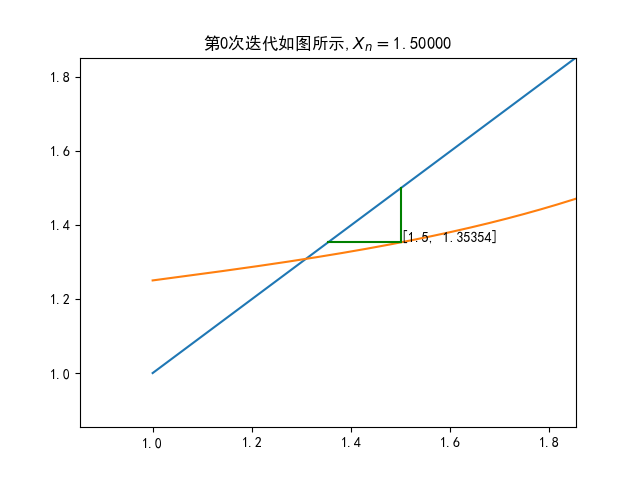
\includegraphics[width=\linewidth]{第0次迭代.png}
  \end{minipage}%
  \begin{minipage}[t]{0.4\linewidth}
  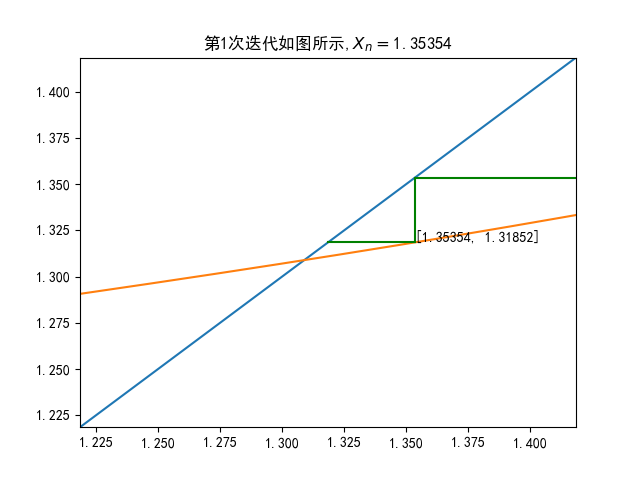
\includegraphics[width=\linewidth]{第1次迭代.png}
  \end{minipage}
\end{figure}

\begin{figure}[h]
  \centering
  \begin{minipage}[t]{0.4\linewidth}
  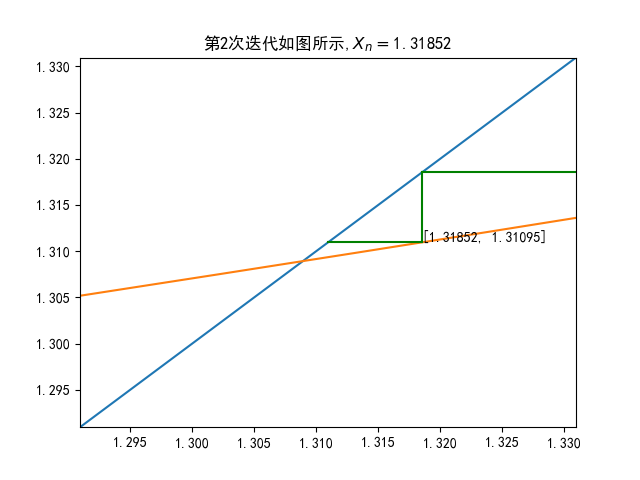
\includegraphics[width=\linewidth]{第2次迭代.png}
  \end{minipage}%
  \begin{minipage}[t]{0.4\linewidth}
  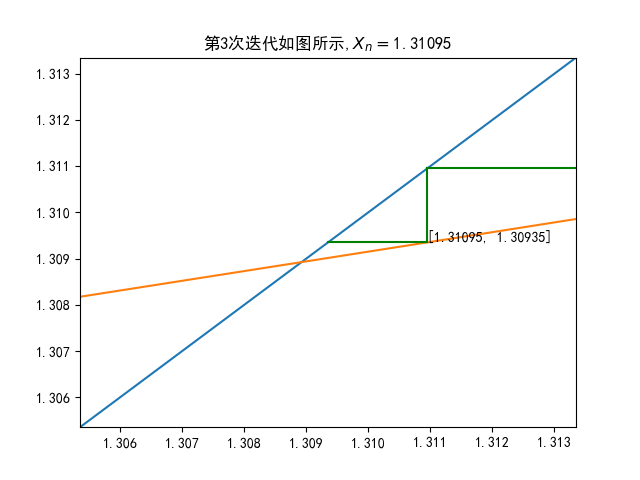
\includegraphics[width=\linewidth]{第3次迭代.png}
  \end{minipage}
\end{figure}

\begin{figure}[h]
  \centering
  \begin{minipage}[t]{0.4\linewidth}
  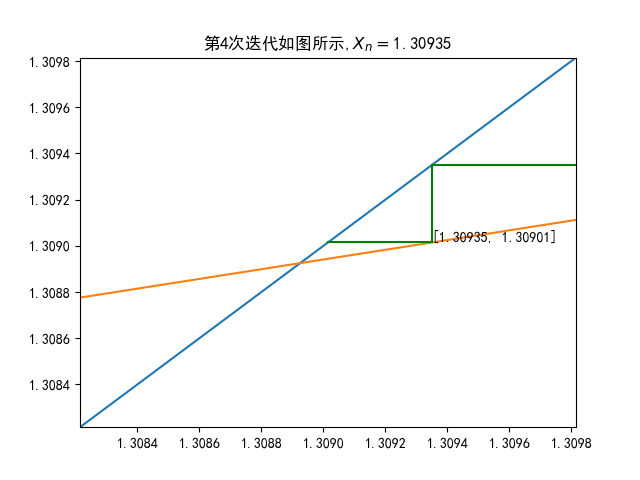
\includegraphics[width=\linewidth]{第4次迭代.png}
  \end{minipage}%
  \begin{minipage}[t]{0.4\linewidth}
  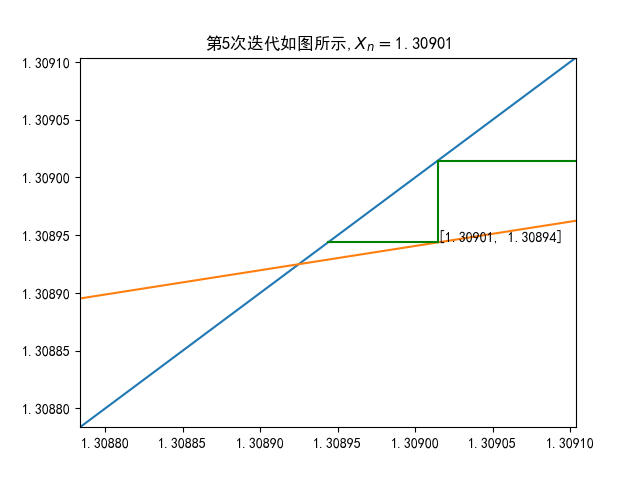
\includegraphics[width=\linewidth]{第5次迭代.png}
  \end{minipage}
\end{figure}
\newpage
\begin{figure}[h]
  \centering
  \begin{minipage}[t]{0.4\linewidth}
  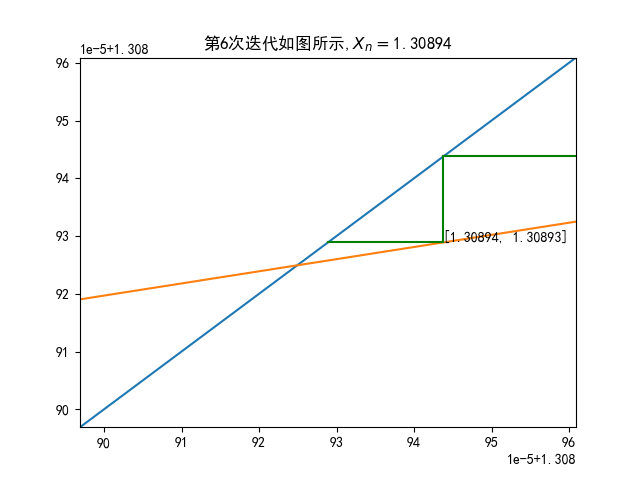
\includegraphics[width=\linewidth]{第6次迭代.png}
  \end{minipage}%
  \begin{minipage}[t]{0.4\linewidth}
  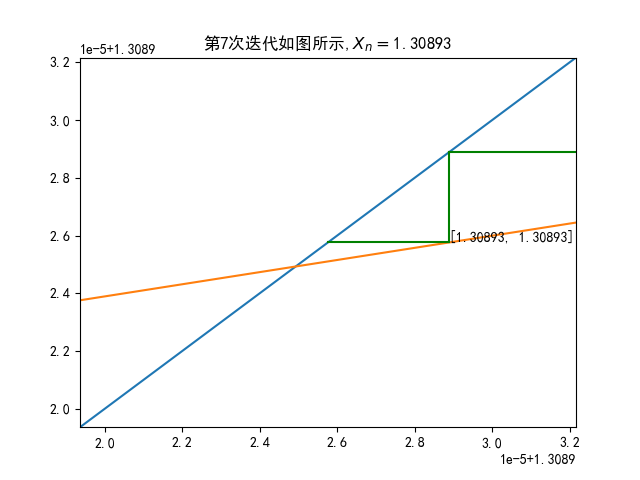
\includegraphics[width=\linewidth]{第7次迭代.png}
  \end{minipage}
\end{figure}
\subsubsection{附录:源代码}
\begin{lstlisting} [language=python]
  import math
  import matplotlib.pyplot as plt
  import numpy as np
  
  plt.rcParams['font.sans-serif'] = ['SimHei']  # 中文字体设置-黑体
  plt.rcParams['axes.unicode_minus'] = False  # 解决保存图像是负号'-'显示为方块的问题
  
  
  #  x = fai5(x)
  
  def f(x):
      return pow((-58 * x - 3) / (7 * pow(x, 3) - 13 * pow(x, 2) - 21 * x - 12), 1 / 2)
  
  
  LIMIT = 1e-5
  xlow = 1
  xup = 2
  xn = 1.5
  tmp = 2
  iter = 0
  points = []
  while math.fabs(xn - tmp) >= LIMIT:  # tmp 表示 x_n-1
      print("{:d} {:.5f}".format(iter, xn))
      iter += 1
      xn, tmp = f(xn), xn
      points.append([tmp, xn])
  print("{:d} {:.5f}".format(iter, xn))
  
  
  i = 0
  a = 0.5
  x0 = np.linspace(1, 2, 100)
  y0 = np.linspace(1, 2, 100)
  plt.plot(x0, y0)
  x1 = np.linspace(1, 2, 10000)
  y1 = np.array([f(t) for t in x1])
  plt.plot(x1, y1)
  for x, y in points:
      plt.title("第{:d}次迭代如图所示,$X_n=${:.5f}".format(i, round(x, 5)))
  
      result_x = round(x, 5)
      result_y = round(y, 5)
      plt.plot([x, x], [x, y], 'g')
      plt.text(x, y, [result_x, result_y])
      plt.pause(1)
      plt.xlim(y - a, y + a)
      plt.ylim(y - a, y + a)
      plt.plot([x, y], [y, y], 'g')
      # plt.savefig('./第{}次迭代.png'.format(i))
      plt.pause(1)
      a = a / 5
      i += 1
\end{lstlisting}

\subsection{Aitken和Steffensen方法加速求根}
\subsubsection{实验题目}
编写Aitken和Steffensen方法加速例2.2的5种迭代格式的结果,写成分析报告(计算结果输出到文件,精度要求为1e-5)
\subsubsection{算法介绍}
$Aitken$方法:

对于一个收敛到$p$的数列${x_n}$ ,如果其收敛阶为1,那么
$$
\lim _{n \rightarrow \infty} \frac{\left|x_{n+1}-p\right|}{\left|x_{n}-p\right|}=C, 0<C<1
$$
可以认为当$n \rightarrow \infty$时,有
$$
\frac{x_{n}-p}{x_{n-1}-p} \approx \frac{x_{n-1}-p}{x_{n-2}-p}
$$
解得
$$
p \approx x_{n}-\frac{\left(x_{n}-x_{n-1}\right)^{2}}{x_{n}-2 x_{n-1}+x_{n-2}}
$$
得到迭代数列
$$
\hat{x}_{n}=x_{n}-\frac{\left(x_{n}-x_{n-1}\right)^{2}}{x_{n}-2 x_{n-1}+x_{n-2}} \stackrel{\text { 或者 }}{=} x_{n-2}-\frac{\left(x_{n-1}-x_{n-2}\right)^{2}}{x_{n}-2 x_{n-1}+x_{n-2}}, n=2,3, \mathrm{~L}
$$
称${x_n}$为Aitken数列,其中$\hat{x}_0=x_0, \hat{x}_1=x_1$。

\quad

算法思路:

已知初值为$x_0$, 第一步, 先求出$x_1=\phi(x_0)$, 可得$\hat{x}_1 = x_1$;

第二步,先求出$x_2\phi(x_1)$, 由迭代数列得
$$
\hat{x}_{2}=x_{0}-\frac{\left(x_{1}-x_{0}\right)^{2}}{x_{2}-2 x_{1}+x_{0}}
$$

第三步,先求出$x_3=\phi(x_2)$,由迭代数列得
$$
\hat{x}_{3}=x_{1}-\frac{\left(x_{2}-x_{1}\right)^{2}}{x_{3}-2 x_{2}+x_{1}}
$$

$Steffensen$方法:
$$
x_{n}=\psi\left(x_{n-1}\right)=x_{n-1}-\frac{\left[\varphi\left(x_{n-1}\right)-x_{n-1}\right]^{2}}{\varphi\left(\varphi\left(x_{n-1}\right)\right)-2 \varphi\left(x_{n-1}\right)+x_{n-1}}
$$
由上式产生的序列称为Steffensen迭代序列。

\quad

算法思路:

已知初值为$x_0$, 第一步,从$x_0$开始迭代,由Steffensen迭代序列得
$$
\hat{x}_{1}=x_{0}-\frac{\left[\varphi\left(x_{0}\right)-x_{0}\right]^{2}}{\varphi\left(\varphi\left(x_{0}\right)\right)-2 \varphi\left(x_{0}\right)+x_{0}}
$$

第二步,从$\hat{x}_1$开始迭代,由Steffensen迭代序列得
$$
\hat{x}_{2}=\hat{x}_{1}-\frac{\left[\varphi\left(\hat{x}_{1}\right)-\hat{x}_{1}\right]^{2}}{\varphi\left(\varphi\left(\hat{x}_{1}\right)\right)-2 \varphi\left(\hat{x}_{1}\right)+\hat{x}_{1}}
$$

以此类推,直到迭代停止。
\subsubsection{实验结果及分析}
\begin{longtable}{cccccc}
  \caption{Aitken方法迭代过程数据}\\ \hline
  迭代次数$n$ & (1) & (2)& (3)& (4)& (5)\\
  \hline
  0 & 1.50000 & 1.50000 & 1.50000 & 1.50000 & 1.50000\\
  1	&1.50002&1.02102 &-2.10438 &1.30825&	1.30751\\
  2	&0	    &0.307844&2.76904	 &1.30889&	1.30887\\
  3	&$\dots$&-15.7335&2.76685	 &1.30892&	1.30892\\
  4 & & 4.32142& & & \\
  5 & &3.2787 & & & \\
  6 & &2.99777 & & & \\
  7 & &2.88398 & & & \\
  8 & &2.82991 & & & \\
  9 & &2.80201 & & & \\
  10 & &2.78689 & & & \\
  11& &2.77845 & & & \\
  12 & &2.77363 & & & \\
  13 & &2.77085 & & & \\
  14 & &2.76922 & & & \\
  15 & &2.76826 & & & \\
  16 & &2.76769 & & & \\
  17 & &2.76735 & & & \\
  18 & &2.76715 & & & \\
  19 & &2.76703 & & & \\
  20 & &2.76696 & & & \\
  21 & &2.76691 & & & \\
  22 & &2.76689 & & & \\
  \hline       
\end{longtable}

\begin{longtable}{cccccc}
  \caption{Steffensen方法迭代过程数据}\\ \hline
  迭代次数$n$ & (1) & (2)& (3)& (4)& (5)\\
  \hline
  0 & 1.50000 & 1.50000 & 1.50000 & 1.50000 & 1.50000\\
  1	&1.50002&1.02102 &-2.10438 &1.30825&	1.30751\\
  2	&1.50004&1.38449+0.543174j&2.65482&1.30892&1.30892\\
  3	&1.50007&1.94712-0.0143892j&2.76673&1.30892&1.30892\\
  4 &1.50009&3.47192+0.0760038j&2.76685 & & \\
  5 &1.50011&2.81754+0.00840694j & & & \\
  6 &1.50013 &2.76729+0.000146022j & & & \\
  7 &1.50015 &2.76685+2.38983e-08j & & & \\
  8 &1.50018 & & & & \\
  $\dots$ & $\dots$& & & &\\
  3213320&2.76685 & & & &\\
  \hline       
\end{longtable}
\subsubsection{附录:源代码}
\begin{lstlisting} [language=python]
def f(x):
  return 7 * x ** 5 - 13 * x ** 4 - 21 * x ** 3 - 12 * x ** 2 + 58 * x + 3


def phi1(x):
  return 7 * x ** 5 - 13 * x ** 4 - 21 * x ** 3 - 12 * x ** 2 + 59 * x + 3


def phi2(x):
  return ((13 * x ** 4 + 21 * x ** 3 + 12 * x ** 2 - 58 * x - 3) / 7) ** (1 / 5)


def phi3(x):
  return (13 + (21 / x) + (12 / (x ** 2)) - (58 / (x ** 3)) - (3 / (x ** 4))) / 7


def phi4(x):
  return ((12 * x ** 2 - 58 * x - 3) / (7 * x ** 2 - 13 * x - 21)) ** (1 / 3)


def phi5(x):
  return ((-58 * x - 3) / (7 * x ** 3 - 13 * x ** 2 - 21 * x - 12)) ** (1 / 2)


def Steffensen(x0, iternum, g, epsilon=1e-5):
  result = []
  with open("Steffensen.txt", "a+") as file:
      for i in range(iternum):
          if (g(g(x0)) - 2 * g(x0) + x0) != 0:
              x1_hat = x0 - (g(x0) - x0) ** 2 / (g(g(x0)) - 2 * g(x0) + x0)

              result.append(x1_hat)
              print("{:d}\t{:.6g}".format(i + 1, x1_hat))  # 第一列:迭代次数 第二列:迭代过程数据
              file.writelines("{:d}\t{:.6g}\n".format(i + 1, x1_hat))
              if abs(x1_hat - g(x1_hat)) < epsilon:
                  return result, x1_hat
              else:
                  x0 = x1_hat
          else:
              print("Steffensen方法失败")
              return None

  print("Steffensen方法失败")
  return None


def Aitken(x0, iternum, g, epsilon=1e-5):
  try:
      with open("Aitken.txt", "a+") as file:
          for i in range(iternum):
              x1 = g(x0)
              x2 = g(x1)
              # print(x1,x2)
              if (x2 - 2 * x1 + x0) != 0:
                  x2_hat = x2 - (x2 - x1) ** 2 / (x2 - 2 * x1 + x0)
                  print("{:d}\t{:.6g}".format(i + 1, x2_hat))  # 第一列:迭代次数 第二列:迭代过程数据
                  file.writelines("{:d}\t{:.6g}\n".format(i + 1, x2_hat))
                  if abs(x2_hat - g(x2_hat)) < epsilon:
                      return x2_hat
                  else:
                      x0 = x1
              else:
                  print("Aitken方法失败")
                  return None
          print("Aitken方法失败")

      return None
  except OverflowError:
      print("溢出")
  except ZeroDivisionError:
      print("分母为零")


if __name__ == '__main__':
  x0 = 1.5  # 迭代初值
  LIMIT = 1e-5  # 精度
  iternum = 10000  # 最大迭代次数

  # Aitken
  print("Atiken1:")
  root1 = Aitken(x0, iternum, phi1)
  print("Atiken2:")
  root2 = Aitken(x0, iternum, phi2)
  print("Atiken3:")
  root3 = Aitken(x0, iternum, phi3)
  print("Atiken4:")
  root4 = Aitken(x0, iternum, phi4)
  print("Atiken5:")
  root5 = Aitken(x0, iternum, phi5)
  # Steffensen
  print("Steffensen1:")
  roots1 = Steffensen(x0, iternum, phi1)
  print("Steffensen2:")
  roots2 = Steffensen(x0, iternum, phi2)
  print("Steffensen3:")
  roots3 = Steffensen(x0, iternum, phi3)
  print("Steffensen4:")
  roots4 = Steffensen(x0, iternum, phi4)
  print("Steffensen5:")
  roots5 = Steffensen(x0, iternum, phi5)
\end{lstlisting}

\subsection{综合实验:多种方法对比}
\subsubsection{实验题目}
采用二分法、不动点迭代法、加速收敛方法、牛顿法、弦截法对例2.1方程进行求解。
列出求解数据表格,并分析。(注意初始值的设置尽量相同)
\subsubsection{算法介绍}
牛顿法:

解非线性方程$f(x) = 0$的牛顿法是一种将非线性函数线性化的方法。取初值
$x_0\approx p$,将$f(x)$做一阶泰勒展开:
$$
f(x)=f\left(x_{n}\right)+f^{\prime}\left(x_{n}\right)\left(x-x_{n}\right)+\frac{f^{\prime \prime}(\xi)}{2 !}\left(x-x_{n}\right)^{2}, \xi \in\left[x_{n}, x\right]
$$

去掉2阶及2阶以上项(即线性化),则有
$$
f(x) \approx f\left(x_{n}\right)+f^{\prime}\left(x_{n}\right)\left(x-x_{n}\right)
$$

$\text { 设 } f^{\prime}\left(x_{n}\right) \neq 0 \text {, 用 } x_{n+1} \text { 代替 } x \text {, 由 } f(x)=0 \text { 得迭代公式 }$
$$
x_{n+1}=x_{n}-\frac{f\left(x_{n}\right)}{f^{\prime}\left(x_{n}\right)}
$$
使用此迭代公式的求根算法称为牛顿法。

\quad

定端点弦截法:

给定$x_0$和$x_1$的值,对于$n=1, 2, K$有
$$
x_{n+1}=x_{n}-\frac{x_{n}-x_{0}}{f\left(x_{n}\right)-f\left(x_{0}\right)} f\left(x_{n}\right)
$$
使用此迭代公式的求根算法称为定端点弦截法。

\quad

动端点弦截法:

给定$x_0$和$x_1$的值,对于$n=1, 2, K$有
$$
x_{n+1}=x_{n}-\frac{x_{n}-x_{n-1}}{f\left(x_{n}\right)-f\left(x_{0}\right)} f\left(x_{n}\right)
$$
使用此迭代公式的求根算法称为动端点弦截法。
\subsubsection{实验结果及分析}
\begin{center}
  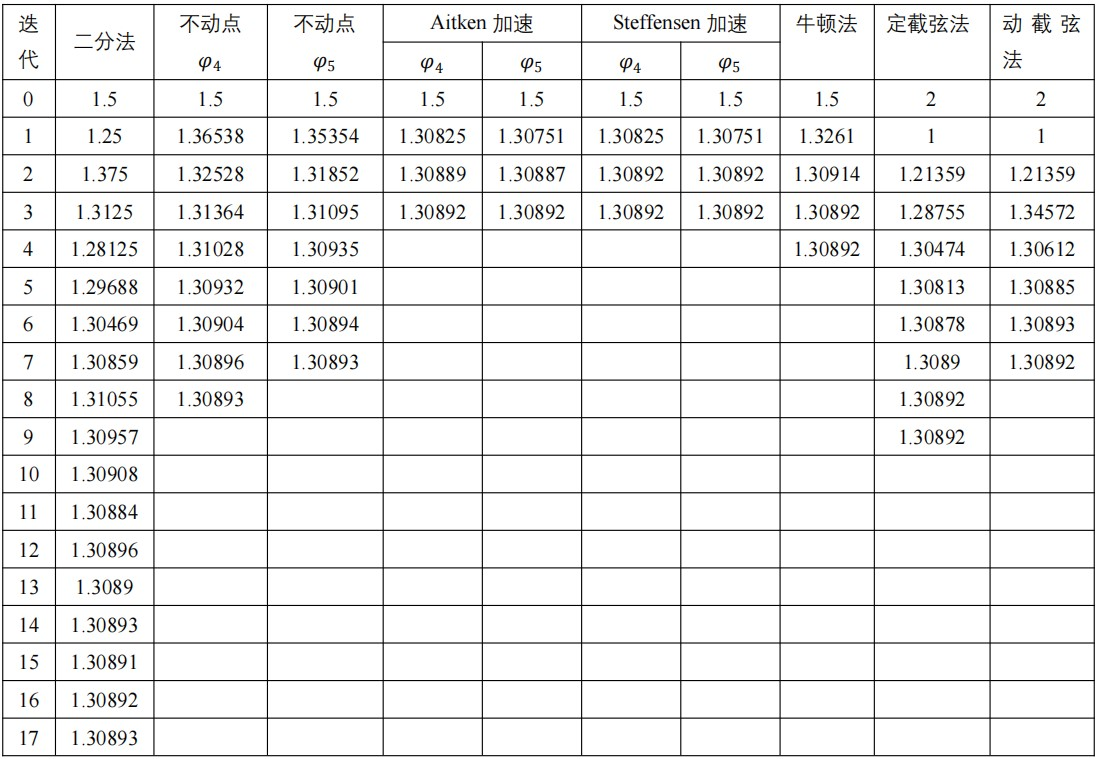
\includegraphics[scale=0.5]{test.jpg}
\end{center}
\subsubsection{附录:源代码}
牛顿法:
\begin{lstlisting} [language=python]
  import math
  from time import *
  
  
  #  x = fai5(x)
  
  def f(x):  # 使用秦九韶算法减少运算次数
      coefficient = [7, -13, -21, -12, 58, 3]
      f = coefficient[0]
      for i in range(1, len(coefficient)):
          f = f * x + + coefficient[i]
      return f
  
  
  def diff_f(x):
      coefficient = [35, -52, -63, -24, 58]
      f = coefficient[0]
      for i in range(1, len(coefficient)):
          f = f * x + + coefficient[i]
      return f
  
  
  LIMIT = 1e-5
  xlow = 1
  xup = 2
  xn = 1.5
  tmp = 2
  iter = 0
  
  while math.fabs(xn - tmp) >= LIMIT:     # tmp 表示 x_n-1
      print("{:d} {:.5f}".format(iter, xn))
      iter += 1
      xn, tmp = xn - f(xn) / diff_f(xn), xn
  print("{:d} {:.5f}".format(iter, xn))  
\end{lstlisting}

\quad

定截弦法:
\begin{lstlisting} [language=python]
  import math
  from time import *
  
  
  #  x = fai5(x)
  
  def f(x):  # 使用秦九韶算法减少运算次数
      coefficient = [7, -13, -21, -12, 58, 3]
      f = coefficient[0]
      for i in range(1, len(coefficient)):
          f = f * x + + coefficient[i]
      return f
  
  
  LIMIT = 1e-5
  x0 = 1
  xn = 2
  tmp = 1.5
  iter = 1
  print("{:d} {:.5f}".format(0, 1))
  while math.fabs(xn - tmp) >= LIMIT:     # tmp 表示 x_n-1
      print("{:d} {:.5f}".format(iter, xn))
      iter += 1
      xn, tmp = xn - ((xn - x0) / (f(xn) - f(x0))) * f(xn), xn
  print("{:d} {:.5f}".format(iter, xn))  
\end{lstlisting}

\quad

动截弦法:
\begin{lstlisting} [language=python]
  import math
  from time import *
  
  
  #  x = fai5(x)
  
  def f(x):  # 使用秦九韶算法减少运算次数
      coefficient = [7, -13, -21, -12, 58, 3]
      f = coefficient[0]
      for i in range(1, len(coefficient)):
          f = f * x + + coefficient[i]
      return f
  
  
  LIMIT = 1e-5
  xn = 2
  tmp = 1
  iter = 1
  print("{:d} {:.5f}".format(0, 1))
  while math.fabs(xn - tmp) >= LIMIT:     # tmp 表示 x_n-1
      print("{:d} {:.5f}".format(iter, xn))
      iter += 1
      xn, tmp = xn - ((xn - tmp) / (f(xn) - f(tmp))) * f(xn), xn
  print("{:d} {:.5f}".format(iter, xn))  
\end{lstlisting}

\newpage

\section{线性方程组的数值解法实验与分析}
\subsection{$Gauss$消去法与列主元$Gauss$消去法的比较}
\subsubsection{实验题目}
$$
  \left\{\begin{aligned}
      2.51 x_{1}+1.48 x_{2}+4.53 x_{3} &=0.05 \\
      1.48 x_{1}+0.93 x_{2}-1.3 x_{3} &=1.03 \\
      2.68 x_{1}+3.04 x_{2}-1.48 x_{3} &=-0.53
      \end{aligned}\right.
$$

(1)使用$Gauss$消去法解以上方程组;

(2)使用列主元$Gauss$消去法解以上方程组;

(3)检验(1)和(2)中得到的两个解中,哪一个更接近准确解。


(计算过程中保留三位小数,方程的准确解为$x_1=1.4530$, $x_2=-1.589195$, $x_3=-0.2748947$)
\subsubsection{算法介绍}
$Gauss$消元法:

消元公式: $(k=1,2, \cdots, n-1)$
$$
    \begin{aligned}
        &l_{i k}=a_{i k}^{(k)} / a_{k k}^{(k)} \quad(i=k+1, \ldots, n) \\
        &\left\{\begin{array}{l}
        a_{i j}^{(k+1)}=a_{i j}^{(k)}-l_{i k} a_{k j}^{(k)} \\
        b_{i}^{(k+1)}=b_{i}^{(k)}-l_{i k} b_{k}^{(k)}
        \end{array} \quad(i, j=k+1, \ldots, n)\right.
        \end{aligned}
$$

回代过程:
$$
    \left\{\begin{array}{l}
        x_{n}=b_{n}^{(n)} / a_{n n}^{(n)} \\
        x_{i}=\frac{b_{i}^{(i)}-\sum_{j=i+1}^{n} a_{i j}^{(i)} x_{j}}{a_{i i}^{(i)}} \quad(i=n-1, \ldots, 1)
        \end{array}\right.
$$

\quad

列主元$Gauss$消去法:

每次消元前选出待消元(按列)的未知数对应的系数中绝对值最大的元素为主元素,然后交换两行后再消元。

Step $k:$ 

(1) 选取 $\left|\boldsymbol{a}_{i_{k}, k}\right|=\max _{k \leq i \leq n}\left|\boldsymbol{a}_{i k}\right| \neq 0$

(2) If $i_{k} \neq k$ then 交换第 $k$ 行与第 $i_{k}$ 行;

(3) 消元 (消元过程即$Gauss$消去法)

消元完回代即可求解出$x$。
\subsubsection{问题求解与分析}
(1):
\begin{equation}\nonumber
    [A|b]=\left[\begin{array}{cccc}
        2.51 & 1.48 & 4.53 & 0.05 \\
        0 & 0.057 & -3.973 & 1.0 \\
        0 & 0 & 95.375 & -26.179
        \end{array}\right]
\end{equation}
回代得: $x_1 = 1.431$, $x_2 = -1.554$, $x_3 = -0.274$。

(2):
\begin{equation}\nonumber
    [A|b]=\left[\begin{array}{cccc}
        2.68 & 3.04 & -1.48 & -0.53 \\
        0 & -1.368 & 5.917 & 0.547 \\
        0 & 0 & -3.72 & 1.024
        \end{array}\right]
\end{equation}
回代得: $x_1 = 1.453$, $x_2 = -1.589$, $x_3 = -0.275$。

\subsubsection{算法源代码}
$Gauss$消去法:
\begin{lstlisting} [language=python]
  # Gauss消去法解方程组
  for k in range(0, n - 1):
      for i in range(k + 1, n):
          l = round(aug_matrix[i][k] / aug_matrix[k][k], 3)
          for j in range(k + 1, n + 1):
              aug_matrix[i][j] = round(aug_matrix[i][j] - l * aug_matrix[k][j], 3)
          aug_matrix[i][k] = 0
  
  for a in aug_matrix:
      print(a)
  print()
  x = [0.0] * n
  
  x[n - 1] = aug_matrix[n - 1][n] / aug_matrix[n - 1][n - 1]
  
  for k in range(n - 1, -1, -1):
      sum = 0
      for j in range(k + 1, n):
          sum += aug_matrix[k][j] * x[j]
      x[k] = round((aug_matrix[k][n] - sum) / aug_matrix[k][k], 3)
  print(x)
  print()
\end{lstlisting}

\quad

列主元$Gauss$消去法:

\begin{lstlisting} [language=python]
  # 列主元Gauss消去法解方程组
  aug_matrix = copy.deepcopy(tmp)
  
  
  def swap(k, n):
      global aug_matrix
      ans = -1
      maxn = -1
      for i in range(k, n):
          if ans < math.fabs(aug_matrix[i][k]):
              ans = math.fabs(aug_matrix[i][k])
              maxn = i
      if maxn == k:
          return
      aug_matrix[k][k::], aug_matrix[maxn][k::] = aug_matrix[maxn][k::], aug_matrix[k][k::]
  
  
  for k in range(0, n - 1):
      swap(k, n)
      for i in range(k + 1, n):
          l = round(aug_matrix[i][k] / aug_matrix[k][k], 3)
          for j in range(k + 1, n + 1):
              aug_matrix[i][j] = round(aug_matrix[i][j] - l * aug_matrix[k][j], 3)
          aug_matrix[i][k] = 0
  
  for a in aug_matrix:
      print(a)
  print()
  x = [0.0] * n
  
  x[n - 1] = aug_matrix[n - 1][n] / aug_matrix[n - 1][n - 1]
  
  for k in range(n - 1, -1, -1):
      sum = 0
      for j in range(k + 1, n):
          sum += aug_matrix[k][j] * x[j]
      x[k] = round((aug_matrix[k][n] - sum) / aug_matrix[k][k], 3)
  print(x)
  
\end{lstlisting}
\subsection{列主元$Gauss-Jordan$消去法、$LU$分解法的对比}
\subsubsection{实验题目}
用列主元$Gauss-Jordan$消去法、$LU$分解法解方程组$Ax = b$

$$
  A=\left[\begin{array}{cccc}
      1 & 2 & 1 & -2 \\
      2 & 5 & 3 & -2 \\
      -2 & -2 & 3 & 5 \\
      1 & 3 & 2 & 3
  \end{array}\right], \quad b=(4,7,-1,0)^{\mathrm{T}}
$$
\subsubsection{算法介绍}
列主元$Gauss-Jordan$消去法:

与$Gauss$消去法的主要区别:

每步不计算 $l_{i k}$, 而是先将当前主元 $a_{k k}{ }^{(k)}$ 变为 1

把 $a_{k k}{ }^{(k)}$ 所在列的上、下元素全消为 0

$A \vec{x}=\vec{b} \Rightarrow I \vec{x}=A^{-1} \vec{b}$

\quad

$LU$分解法:

$\boldsymbol{A} \overrightarrow{\boldsymbol{x}}=\boldsymbol{L} \boldsymbol{U} \overrightarrow{\boldsymbol{x}}=\overrightarrow{\boldsymbol{b}}_{i} \quad(i=1,2, \cdots, k)$

令 $U \vec{x}=\vec{y}$ ,则 $L \vec{y}=\vec{b}_{i}$

解出 $\vec{y}$ 代入上式即得 $\overrightarrow{\boldsymbol{x}}$ ,那么解方程组变成相继解 两个三角方程组。

对于$\boldsymbol{L} \overrightarrow{\boldsymbol{y}}=\overrightarrow{\boldsymbol{b}}_{i}$

有$y_{i}=b_{i}-\sum_{k=1}^{i-1} l_{i k} y_{k} \quad i=1,2, \cdots, n$

对于$\boldsymbol{U} \overrightarrow{\boldsymbol{x}}=\overrightarrow{\boldsymbol{y}}$

有$x_{i}=\left(y_{i}-\sum_{k=i+1}^{n} u_{i k} x_{k}\right) / u_{i i} \quad i=n, n-1, \cdots, 1$

\subsubsection{问题求解与分析}
列主元$Gauss-Jordan$消去法:
$$
  [A \mid b]=\left[\begin{array}{ccccc}
      1 & 0 & 0 & 0 & 2 \\
      0 & 1 & 0 & 0 & -1 \\
      0 & 0 & 1 & 0 & 2 \\
      0 & 0 & 0 & 1 & -1
      \end{array}\right]
$$
得:  $x=(2,-1,2,-1)^{\mathrm{T}}$ 。

\quad

$LU$分解法:
$$
  [U \mid y]=\left[\begin{array}{ccccc}
      1 & 2 & 1 & -1 & 4 \\
      0 & 1 & 1 & 2 & -1 \\
      0 & 0 & 3 & -3 & 9 \\
      0 & 0 & 0 & 3 & -3
      \end{array}\right]
$$
得:  $x=(2,-1,2,-1)^{\mathrm{T}}$ 。

列主元$Gauss-Jordan$消去法比$Gauss$消去法多出 $O(\frac{n^2}{3})$的比较步骤

$LU$分解法总计算量为
\begin{equation}\nonumber
    \frac{n^{3}+3 n^{2}-n}{3}
\end{equation}

与$Gauss$消去法相同
\subsubsection{算法源代码}
列主元$Gauss-Jordan$消去法:
\begin{lstlisting} [language=python]
  # 列主元Gauss-Jordan消去法
  def swap(k, n):
      global aug_matrix
      ans = -1
      maxn = -1
      for i in range(k, n):
          if ans < math.fabs(aug_matrix[i][k]):
              ans = math.fabs(aug_matrix[i][k])
              maxn = i
      if maxn != k:
          aug_matrix[k][k::], aug_matrix[maxn][k::] = aug_matrix[maxn][k::], aug_matrix[k][k::]
      l = aug_matrix[k][k]
      for j in range(k, n + 1):
          aug_matrix[k][j] /= l
  
  
  for k in range(0, n):
      swap(k, n)
      for i in range(0, n):
          if i == k:
              continue
          l = round(aug_matrix[i][k] / aug_matrix[k][k], 3)
          for j in range(k + 1, n + 1):
              aug_matrix[i][j] = round(aug_matrix[i][j] - l * aug_matrix[k][j], 3)
          aug_matrix[i][k] = 0
  
  for a in aug_matrix:
      print(a)
  print()
  
  x = [0.0] * n
  
  for i in range(n):
      x[i] = aug_matrix[i][n]
  print('列主元Gauss-Jordan消去法:')
  print(x)
\end{lstlisting}

\quad

$LU$分解法:
\begin{lstlisting} [language=python]
  # LU分解法解方程组
  aug_matrix = copy.deepcopy(tmp)
  L = [[0.0] * n for _ in range(n)]
  for k in range(n-1):
      for i in range(k+1, n):
          L[i][k] = aug_matrix[i][k] / aug_matrix[k][k]
          for j in range(n):
              aug_matrix[i][j] = aug_matrix[i][j] - L[i][k] * aug_matrix[k][j]
  for i in range(n):
      L[i][i] = 1.0
  
  # 求 y
  y = [0.0] * n
  y[0] = aug_matrix[0][n]
  for i in range(1, n):
      y[i] = aug_matrix[i][n]
      for j in range(i):
          y[i] = y[i] - L[i][j] * y[j]
  # print(y)
  
  # aug_matrix 为ux=y 的增广矩阵
  for i in range(n):
      aug_matrix[i][n] = y[i]
  
  for a in aug_matrix:
      print(a)
  print()
  # 求x
  x = [0.0] * n
  x[n - 1] = aug_matrix[n - 1][n] / aug_matrix[n - 1][n - 1]
  
  for k in range(n - 1, -1, -1):
      sum = 0
      for j in range(k + 1, n):
          sum += aug_matrix[k][j] * x[j]
      x[k] = round((aug_matrix[k][n] - sum) / aug_matrix[k][k], 3)
  print('LU分解法解方程组:')
  print(x)
  print()
\end{lstlisting}

\subsection{范数和条件数的求解}
\subsubsection{实验题目}
求出
$$
    \boldsymbol{A}=\left[\begin{array}{cccc}
        -2 & 1 & 0 & 0 \\
        1 & -2 & 1 & 0 \\
        0 & 1 & -2 & 1 \\
        0 & 0 & 1 & -2
        \end{array}\right]
$$

的$\|A\|_{\infty},\|A\|_{1},\|A\|_{2} \text { 和 } \operatorname{Cond}(A)_{2}$
\subsubsection{预备知识}
$\|A\|_{1}=\max _{1 \leq i \leq n} \sum_{j=1}^{n}\left|a_{i j}\right|$ (行和范数)

$\|A\|_{1}=\max _{1 \leq j \leq n} \sum_{i=1}^{n}\left|a_{i j}\right|$ (列和范数)

$\|\boldsymbol{A}\|_{2}=\sqrt{\rho\left(\boldsymbol{A}^{\mathrm{T}} \boldsymbol{A}\right)} \quad$ (谱范数 /* spectral norm */ )

$\operatorname{cond}(A)_{2}=\sqrt{\lambda_{\max }\left(A^{T} A\right) / \lambda_{\min }\left(A^{T} A\right)}$

\subsubsection{问题求解与分析}
$\|{A}\|_{\infty} = 4 $

$\|A\|_{1} = 4$

$\|{A}\|_{2} = 3.6180339887498953$

$\operatorname{Cond}(A)_{2} = 9.472135954999562$
\subsubsection{算法源代码}
\begin{lstlisting} [language=python]
  import math
  from math import inf
  import numpy as np
  
  A = np.array([[-2, 1, 0, 0], [1, -2, 1, 0], [0, 1, -2, 1], [0, 0, 1, -2]])
  
  # inf 范数
  norm_inf = 0
  for i in range(A.shape[0]):
      tmp = 0
      for j in range(A.shape[1]):
          tmp += abs(A[i][j])
      if tmp > norm_inf:
          norm_inf = tmp
  print(norm_inf)
  # print(np.linalg.norm(A, ord=inf))
  
  # 1 范数
  norm_1 = 0
  for j in range(A.shape[1]):
      tmp = 0
      for i in range(A.shape[0]):
          tmp += abs(A[i][j])
      if tmp > norm_1:
          norm_1 = tmp
  print(norm_1)
  # print(np.linalg.norm(A, ord=1))
  
  # 2 范数
  eig, eig_vector = np.linalg.eig(np.dot(A.T, A))    # 特征值, 特征向量
  norm_2 = math.sqrt(max(eig))
  print(norm_2)
  # print(np.linalg.norm(A, ord=2))
  
  # Cond(A)_2
  CondA = math.sqrt(max(eig)) / math.sqrt(min(eig))
  print(CondA)
\end{lstlisting}

\subsection{微小扰动对方程组求解的稳定性分析}
\subsubsection{实验题目}
解如下方程组

$$
    \left[\begin{array}{cccc}
        10 & 7 & 8 & 7 \\
        7 & 5 & 6 & 5 \\
        8 & 6 & 10 & 9 \\
        7 & 5 & 9 & 10
        \end{array}\right] x=b
$$

其中 $\boldsymbol{b}=(32,23,33,31)^{\mathrm{T}}$, 
但是由于某些原因使得方程的右端被修改为 $b^{*}=(32.1,22.9,33.1,30.9)^{\mathrm{T}}$,
求出方程的解, 并算出在 $\infty$-范数和 1-范数下求出的解与准确解 之间、
扰动方程的右端项和原右端项的相对误差, 说明原因。
\subsubsection{预备知识}
解与准确解的相对误差:
\begin{equation}\nonumber
\begin{split}
    \delta \bar{x}=\vec{x}^{*}-\vec{x}\Rightarrow \frac{\|\delta \vec{x}\|_{\infty}}{\|\vec{x}\|_{\infty}}\\
    \delta \bar{x}=\vec{x}^{*}-\vec{x}\Rightarrow \frac{\|\delta \vec{x}\|_{1}}{\|\vec{x}\|_{1}}
\end{split}
\end{equation}

扰动方程的右端项和原右端项的相对误差:
\begin{equation}\nonumber
    \begin{split}
        \delta \bar{b}=\vec{b}^{*}-\vec{b}\Rightarrow \frac{\|\delta \vec{b}\|_{\infty}}{\|\vec{b}\|_{\infty}}\\
        \delta \bar{b}=\vec{b}^{*}-\vec{b}\Rightarrow \frac{\|\delta \vec{b}\|_{1}}{\|\vec{b}\|_{1}}
    \end{split}
  \end{equation}
\subsubsection{问题求解与分析}
求得方程的准确解为: $x=(1,1,1,1)^{\mathrm{T}}$

解为: $x^{*}=(9.2,-12.6,4.5,-1.1)^{\mathrm{T}}$

\begin{equation}\nonumber
    \begin{split}
        \frac{\|\delta \vec{x}\|_{\infty}}{\|\vec{x}\|_{\infty}} = 13.5999\\
        \frac{\|\delta \vec{x}\|_{1}}{\|\vec{x}\|_{1}} = 6.8500\\
        \frac{\|\delta \vec{b}\|_{\infty}}{\|\vec{b}\|_{\infty}} = 0.003030\\
        \frac{\|\delta \vec{b}\|_{1}}{\|\vec{b}\|_{1}} = 0.0033613
    \end{split}
\end{equation}

虽然$\frac{\|\delta \vec{b}\|}{\|\vec{b}\|} < 0.01$

但是对于求得的解与准确解之间相对误差极大。
\subsubsection{算法源代码}
\begin{lstlisting} [language=python]
  import numpy as np

  A = np.array([[10, 7, 8, 7], [7, 5, 6, 5], [8, 6, 10, 9], [7, 5, 9, 10]], dtype=float)
  
  b1 = np.array([32, 23, 33, 31])
  b2 = np.array([32.1, 22.9, 33.1, 30.9])
  
  result1 = np.linalg.solve(A, b1)
  print(result1)
  result2 = np.linalg.solve(A, b2)
  print(result2)
  
  # 解与准确解的相对误差
  mis_result = result2 - result1
  print(np.linalg.norm(mis_result, ord=np.inf) / np.linalg.norm(result1, ord=np.inf))
  print(np.linalg.norm(mis_result, ord=1) / np.linalg.norm(result1, ord=1))
  
  
  # 扰动方程的右端项和原右端项的相对误差
  mis_b = b2 - b1
  print(np.linalg.norm(mis_b, ord=np.inf) / np.linalg.norm(b1, ord=np.inf))
  print(np.linalg.norm(mis_b, ord=1) / np.linalg.norm(b1, ord=1))
  
\end{lstlisting}

\subsection{$Jacobi$和$Gauss-Seidel$迭代法收敛性}
\subsubsection{实验题目}
设有系数矩阵
\begin{equation}\nonumber
        (1)\left[\begin{array}{ccc}
            1 & 2 & -2 \\
            1 & 1 & 1 \\
            2 & 2 & 1
            \end{array}\right]
        ~~
        (2)\left[\begin{array}{ccc}
            2 & -1 & 1 \\
            1 & 1 & 1 \\
            1 & 1 & -2
            \end{array}\right]
\end{equation}


分别检验以上系数矩阵用$Jacobi$迭代法和$Gauss-Seidel$迭代法是否收敛
\subsubsection{预备知识}
设有方程组 $\vec{x}=B \vec{x}+\vec{g}$ ,对任意初始向量 $\overrightarrow{\boldsymbol{x}}^{(0)}$ 及任意常数
向量 $\vec{g}$ ,解此方程组的迭代法 
(即 $\vec{x}^{(k+1)}=B \vec{x}^{(k)}+\vec{g}, k \rightarrow \infty$ ) 收敛的充要条件是
$$
\rho(B)<1
$$
其中 $\rho(B)=\max _{1 \leq i \leq n}\left|\lambda_{i}\right| , \lambda_{i}$ 为 $B$ 的特征值。

\subsubsection{问题求解与分析}
$\rho(B_j) = 1.0809e-05$, $\rho(B_s) = 2.0$

系数矩阵1:$Jacobi$迭代法收敛, $Gauss-Seidel$迭代法不收敛。



$\rho(B_j) = 1.118$, $\rho(B_s) = 0.5$

系数矩阵2:$Jacobi$迭代法不收敛, $Gauss-Seidel$迭代法收敛。
\subsubsection{算法源代码}
\begin{lstlisting} [language=python]
  import numpy as np

  A1 = np.mat([[1, 2, -2], [1, 1, 1], [2, 2, 1]])
  A2 = np.mat([[2, -1, 1], [1, 1, 1], [1, 1, -2]])
  
  
  def judge_convergence(B):
      eig, _ = np.linalg.eig(B)
      print(np.max(abs(eig)))
      if np.max(abs(eig)) < 1:
          return True
      else:
          return False
  
  
  def solve(A):
      D = np.mat(np.diag(np.diag(A)))
      L = np.tril(A, -1)
      U = np.triu(A, 1)
      B_j = np.dot(-D.I, L + U)
      B_s = np.dot(-(D + L).I, U)
      print('Jacobi迭代法:', judge_convergence(B_j))
      print('Gauss_Seidel迭代法:', judge_convergence(B_s))
  
  
  solve(A1)
  print()
  solve(A2)
    
\end{lstlisting}
\subsection{$Jacobi$和$Gauss-Seidel$迭代法解方程组}
\subsubsection{实验题目}
\begin{equation}\nonumber
  \left\{\begin{aligned}
      11 x_{1}-3 x_{2}-2 x_{3} &=3 \\
      -x_{1}+5 x_{2}-3 x_{3} &=6 \\
      -2 x_{1}-12 x_{2}+19 x_{3} &=-7
      \end{aligned}\right.
\end{equation}

$\text { 取初值为 }(0,0,0)^{\mathrm{T}} \text {, 写出前 } 3 \text { 次迭代的结果。 }$

\subsubsection{预备知识}
$Jacobi$迭代法:

\begin{equation}\nonumber
    \begin{aligned}
        A \vec{x}=\vec{b} & \Leftrightarrow(D+L+U) \vec{x}=\vec{b} \\
        & \Leftrightarrow D \vec{x}=-(L+U) \vec{x}+\vec{b} \quad (\text { 两边左乘 } D^{-1}) \\
        & \Leftrightarrow \vec{x}^{(k+1)}=-D^{-1}(L+U) \vec{x}^{(k)}+D^{-1} \vec{b}\\
        & \quad\quad{x}^{(k+1)}={B}_{\mathbf{J}} {x}^{(k)}+\vec{g}_{\mathrm{J}}
        \end{aligned}
\end{equation}

\quad

$Gauss-Seidel$迭代法:

\begin{equation}\nonumber
    \begin{aligned}
        &{[L+D+U] x=b} \\
        &D x=-L x-U x+b \\
        &D x^{(k+1)}=-L x^{(k+1)}-U x^{(k)}+b \\
        &\Leftrightarrow(D+L) \vec{x}^{(k+1)}=-U \vec{x}^{(k)}+\vec{b} \\
        &\Leftrightarrow \vec{x}^{(k+1)}=-(D+L)^{-1} U \vec{x}^{(k)}+(D+L)^{-1} \vec{b} \\
        & \quad\quad{x}^{(k+1)}={B}_{\mathbf{s}} {x}^{(k)}+\vec{g}_{\mathrm{s}}
        \end{aligned}
\end{equation}
\subsubsection{问题求解与分析}
$Jacobi$迭代法:

\begin{table}[h]
    \vspace{20pt}
    \centering
    \begin{tabular}{cllll}
        \hline
        迭代次数 & $x_1$& $x_2$ & $x_3$\\
        \hline
        0  & 0.0          & 0.0             & 0.0           \\
        1  & 0.27272727   & 1.2             & -0.36842105   \\
        2  & 0.53301435   & 1.03349282      & 0.41818182    \\
        3  & 0.63062201   & 1.55751196      & 0.34041803    \\
        \hline       
    \end{tabular}
\end{table}

\quad

$Gauss-Seidel$迭代法:
\begin{table}[h]
    \vspace{20pt}
    \centering
    \begin{tabular}{cllll}
        \hline
        迭代次数 & $x_1$& $x_2$ & $x_3$\\
        \hline
        0  & 0.0          & 0.0             & 0.0           \\
        1  & 0.27272727   & 1.25454545      & 0.45263158    \\
        2  & 0.69717268   & 1.61101348      & 0.72244775    \\
        3  & 0.84344872   & 1.80215839      & 0.85856832    \\
        \hline       
    \end{tabular}
\end{table}

分析:
该系数矩阵用$Jacobi$迭代法和$Gauss-Seidel$迭代法均收敛。

且该系数矩阵$Gauss-Seidel$迭代法比$Jacobi$迭代法收敛速度更快。

\subsubsection{算法源代码}
\begin{lstlisting} [language=python]
  import numpy as np

  A = np.mat([[11, -3, -2], [-1, 5, -3], [-2, -12, 19]])
  b = np.mat([3, 6, -7]).reshape(-1, 1)
  
  
  def judge_convergence(B):   # 利用谱半径来判断是否收敛
      eig, _ = np.linalg.eig(B)
      if np.max(abs(eig)) < 1:
          return True
      else:
          return False
  
  
  def Jacobi(A, b):
      D = np.mat(np.diag(np.diag(A)))
      L = np.tril(A, -1)
      U = np.triu(A, 1)
      B_j = np.dot(-D.I, L + U)
      g_j = np.dot(D.I, b)
      if judge_convergence(B_j):
          x = np.mat(np.zeros(shape=(A.shape[0], 1)))
          print('初始值:', x.T)
          for i in range(3):
              x = np.dot(B_j, x) + g_j
              print('第{:d}次迭代:'.format(i+1), x.T)
      else:
          print("此系数矩阵Jacobi迭代法不收敛!")
  
  
  def Gauss_Seidel(A, b):
      D = np.mat(np.diag(np.diag(A)))
      L = np.tril(A, -1)
      U = np.triu(A, 1)
      B_s = np.dot(-(D + L).I, U)
      g_s = np.dot((D + L).I, b)
      if judge_convergence(B_s):
          x = np.mat(np.zeros(shape=(A.shape[0], 1)))
          print('初始值:', x.T)
          for i in range(3):
              x = np.dot(B_s, x) + g_s
              print('第{:d}次迭代:'.format(i+1), x.T)
      else:
          print("此系数矩阵Gauss_Seidel迭代法不收敛!")
  
  
  Jacobi(A, b)
  print()
  Gauss_Seidel(A, b)
\end{lstlisting}
\subsection{综合实验:直接法和迭代法求解病态方程组}
\subsubsection{实验题目}
系数矩阵为$Hilbert$阵,对解全为1的方程组,随着$n = 2,3,……$的增加,
编写程序,测试和分析利用直接法和迭代法求解方程组的结果差别。

\begin{equation}\nonumber
    H_{n}=\left[\begin{array}{cccc}
        1 & \frac{1}{2} & \cdots & \frac{1}{n} \\
        \frac{1}{2} & \frac{1}{3} & \ddots & \vdots \\
        \vdots & \vdots & \ddots & \vdots \\
        \frac{1}{n} & \frac{1}{n+1} & \cdots & \frac{1}{2 n-1}
        \end{array}\right]
\end{equation}
\subsubsection{实验准备}
直接法采用$Gauss$消元法进行求解。

迭代法采用$Jacobi$迭代法,$Gauss_Seidel$迭代法求解。

x 的准确解为$x = (1, 1, 1, \cdots, 1)^{\mathrm{T}}$

利用下式计算各方法所求出的解与准确解之间的误差。
\begin{equation}\nonumber
        \delta \bar{x}=\vec{x}^{*}-\vec{x}\Rightarrow \frac{\|\delta \vec{x}\|_{\infty}}{\|\vec{x}\|_{\infty}}
\end{equation}
\subsubsection{实验结果与分析}
选取$n = 2, 5, 10, 20$进行分析。


\begin{table}[h]
    \vspace{5pt}
    \centering
    \begin{tabular}{lllll}
        \hline
         & 解&误差\\
        \hline
        $Gauss$  & $x = (1.0, 1.0)^{\mathrm{T}}$ &1.1102e-15\\
        $Jacobi$  & $x = (1.0, 1.0)^{\mathrm{T}}$ &1.1339e-07\\
        $Gauss-Seidel$ & $x = (1.0, 1.0)^{\mathrm{T}}$& 7.0790e-07\\
        准确解 & $x = (1, 1)^{\mathrm{T}}$ & \\
        \hline       
    \end{tabular}
    \caption{$n = 2$}
\end{table}
从表1可以看出,n=2时,三种方法求出的解都比较精确,误差极小。
\newpage
\begin{table}[h]
    \vspace{5pt}
    \centering
    \begin{tabular}{lllll}
        \hline
         & 解&误差\\
        \hline
        $Gauss$  & $x = (1.0, 1.0, 1.0, 1.0, 1.0)^{\mathrm{T}}$ &6.23424e-12\\
        $Jacobi$  & 不收敛 &\\
        $Gauss-Seidel$ & $x = (0.99978, 1.00437, 0.98045, 1.03016, 0.98504)^{\mathrm{T}}$& 0.069257\\
        准确解 & $x = (1, 1, 1, 1, 1)^{\mathrm{T}}$ & \\
        \hline       
    \end{tabular}
    \caption{$n = 5$}
\end{table}
从表2可以看出,n=5时,Jacobi不收敛,而Gauss-Seidiel方法误差上升到0.069257,Gauss方法误差仍较小。

\begin{table}[h]
    \vspace{5pt}
    \centering
    \begin{tabular}{lllll}
        \hline
         & 解&误差\\
        \hline
        $Gauss$  & $x = (1.0, 1.0, \cdots, 0.99991, 1.00004, 0.99999)^{\mathrm{T}}$ &3.11177e-4\\
        $Jacobi$  & 不收敛 &\\
        $Gauss-Seidel$ & $x = (0.99688, 1.06466, \cdots, 1.01739, 0.95543, 0.88949)^{\mathrm{T}}$& 0.64467\\
        准确解 & $x = (1, 1, \cdots,1, 1, 1)^{\mathrm{T}}$ & \\
        \hline       
    \end{tabular}
    \caption{$n = 10$}
\end{table}
从表3可以看出,n=10时,Jacobi方法不收敛,而Gauss-Seidel与Gauss方法所求出的解的误差继续上升。

\begin{table}[h]
    \vspace{5pt}
    \centering
    \begin{tabular}{lllll}
        \hline
         & 解&误差\\
        \hline
        $Gauss$  & $x = (1.0, 0.9999, \cdots, 1.23974, 0.99395, 1.03248)^{\mathrm{T}}$ &39.541\\
        $Jacobi$  & 不收敛 &\\
        $Gauss-Seidel$ & 不收敛 &\\
        准确解 & $x = (1, 1, \cdots,1, 1, 1)^{\mathrm{T}}$ & \\
        \hline       
    \end{tabular}
    \caption{$n = 20$}
\end{table}
从表4可以看出,n=20时,Jacobi方法,Gauss-Seidel方法不收敛,而Gauss方法所求出解已经上升至39.541。

\subsubsection{算法源代码}
\begin{lstlisting} [language=python]
  import numpy as np


  def Gauss(aug_matrix):
      for k in range(0, n - 1):
          for i in range(k + 1, n):
              l = aug_matrix[i][k] / aug_matrix[k][k]
              for j in range(k + 1, n + 1):
                  aug_matrix[i][j] = aug_matrix[i][j] - l * aug_matrix[k][j]
              aug_matrix[i][k] = 0
  
      x = np.ones(n)
  
      x[n - 1] = aug_matrix[n - 1][n] / aug_matrix[n - 1][n - 1]
  
      for k in range(n - 1, -1, -1):
          sum = 0
          for j in range(k + 1, n):
              sum += aug_matrix[k][j] * x[j]
          x[k] = (aug_matrix[k][n] - sum) / aug_matrix[k][k]
      print(np.round(x, 5))
      print('误差:', np.linalg.norm(x - x_exact, ord=np.inf) / np.linalg.norm(x_exact, ord=np.inf))
  
  
  def judge_convergence(B):
      eig, _ = np.linalg.eig(B)
      if np.max(abs(eig)) < 1:
          return True
      else:
          return False
  
  
  def Jacobi(A, b):
      D = np.mat(np.diag(np.diag(A)))
      L = np.tril(A, -1)
      U = np.triu(A, 1)
      B_j = np.dot(-D.I, L + U)
      g_j = np.dot(D.I, b)
      if judge_convergence(B_j):
          limit = 1e-7
          x0 = np.mat(np.zeros(shape=(A.shape[0], 1)))
          x = np.dot(B_j, x0) + g_j
          while np.min(abs(x - x0)) > limit:
              x0 = x
              x = np.dot(B_j, x) + g_j
          print(np.round(x.T, 5))
          print('误差:', np.linalg.norm(x.reshape(1, -1) - x_exact, ord=np.inf) / np.linalg.norm(x_exact, ord=np.inf))
      else:
          print("该矩阵不收敛!")
  
  
  def Gauss_Seidel(A, b):
      D = np.mat(np.diag(np.diag(A)))
      L = np.tril(A, -1)
      U = np.triu(A, 1)
      B_s = np.dot(-(D + L).I, U)
      g_s = np.dot((D + L).I, b)
      if judge_convergence(B_s):
          limit = 1e-7
          x0 = np.mat(np.zeros(shape=(A.shape[0], 1)))
          x = np.dot(B_s, x0) + g_s
          while np.min(np.fabs(x - x0)) > limit:
              x0 = x
              x = np.dot(B_s, x) + g_s
          print(np.round(x.T, 5))
          print('误差:', np.linalg.norm(x.reshape(1, -1) - x_exact, ord=np.inf) / np.linalg.norm(x_exact, ord=np.inf))
      else:
          print("该矩阵不收敛!")
  
  
  nums = [2, 5, 10, 20]
  for n in nums:
      print('n =', n)
      x_exact = np.ones(n).reshape(-1, 1)
      Hilbert = np.empty((n, n))
      x = np.ones(n).reshape(-1, 1)
  
      for i in range(0, n):
          for j in range(0, n):
              Hilbert[i][j] = 1 / (j + 1 + i)
      b = np.dot(Hilbert, x)
  
      # Gauss
      Gauss(np.concatenate((Hilbert, b), axis=-1))
  
      # 迭代法
      x = np.mat(np.ones(n).reshape(-1, 1))
      b = np.dot(Hilbert, x)
      print('Jacobi:')
      Jacobi(Hilbert, b)
      print('Gauss_Seidel:')
      Gauss_Seidel(Hilbert, b)
      print()
\end{lstlisting}

\newpage

\section{插值法的实验与分析}
\subsection{综合实验:物体运动轨迹的插值预测}
\subsubsection{实验题目}
采用拉格朗日插值、分段线性插值、样条插值等方法进行插值,估计$x=-3.75$和0.25位置的$y$坐标值,并绘制插值函数的图形
,根据结果,确定一种最好的插值方法。
\subsubsection{算法介绍}
拉格朗日插值法:

构造 $x_{0}, \cdots, x_{n}$处的插值基函数。

对于 $x_{i}$ 的插值基函数 $l_{i}(x)$, 它在 $x_{0}, \cdots, x_{i-1}, x_{i+1}, \cdots, x_{n}$ 上都是零点, 其次数不高于 $n$, 因此可以假设
$$
l_{i}(x)=A\left(x-x_{0}\right) \cdots\left(x-x_{i-1}\right)\left(x-x_{i+1}\right) \cdots\left(x-x_{n}\right)
$$
又由于 $l_{i}(x)$ 在 $x_{i}$ 点上的函数值是 1 , 可以解得
$$
A=\frac{1}{\left(x_{i}-x_{0}\right) \cdots\left(x_{i}-x_{i-1}\right)\left(x_{i}-x_{i+1}\right) \cdots\left(x_{i}-x_{n}\right)}
$$
因此, 有
$$
l_{i}(x)=\frac{\left(x-x_{0}\right) \cdots\left(x-x_{i-1}\right)\left(x-x_{i+1}\right) \cdots\left(x-x_{n}\right)}{\left(x_{i}-x_{0}\right) \cdots\left(x_{i}-x_{i-1}\right)\left(x_{i}-x_{i+1}\right) \cdots\left(x_{i}-x_{n}\right)}, \quad i=1,2, \cdots, n
$$
以 $y_{0}, y_{1}, \cdots, y_{n}$ 作为基函数的组合系数, 得到 $n$ 次拉格朗日插值多项式
$$
L_{n}(x)=\sum_{i=0}^{n} y_{i} l_{i}(x)
$$

$n$次插值的截断误差公式

$$
R(x)=f(x)-\varphi_{n}(x)=\frac{f^{(n+1)}(\xi)}{(n+1) !}\left(x-x_{0}\right)\left(x-x_{1}
\right) \cdots\left(x-x_{n}\right)
$$

\quad

牛顿多项式插值法:

$$
f\left[x_{0}, x_{1}, \cdots, x_{n}\right]=\frac{f\left[x_{0}, x_{1}, \cdots, x_{n-2}, x_{n}\right]-f\left[x_{0}, x_{1}, \cdots, x_{n-2}, x_{n-1}\right]}{x_{n}-x_{n-1}}
$$

为函数 $f(x)$ 在节点 $x_{0}, x_{1}, \ldots, x_{n}$ 处的 $n$ 阶差商

1) 通过已知插值节点的函数值建立差商表

2) 以相应的差商作为系数就可以得到插值多项式

\begin{figure}[h]
    \centering
    \begin{minipage}[t]{0.4\linewidth}
    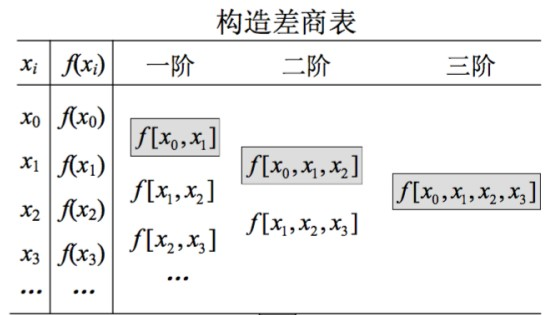
\includegraphics[width=\linewidth]{chashangbiao.jpg}
    \end{minipage}%
\end{figure}
$$
\varphi_{n}(x)=a_{0}+a_{1}\left(x-x_{0}\right)+a_{2}\left(x-x_{0}\right)\left(x-x_{1}\right)+
\cdots+a_{n}\left(x-x_{0}\right)\left(x-x_{1}\right) \cdots\left(x-x_{n-1}\right)
$$
$$a_{i} = f[x_0,x_1,\cdots,x_i]$$

\quad

分段线性插值法:

给定 $n+1$ 个插值节点 $x_{0}<x_{1}<\cdots<x_{n}$ 
以及在这些插值节点上 的函数值 $y_{0}, y_{1}, \cdots, y_{n}$, 构造一个分段插值函数 $P(x)$, 
使得对 任意 $i=0,1,2, \cdots, n$, 有 $P\left(x_{i}\right)=y_{i}$, 
并且在每个子区间 $\left[x_{i}, x_{i+1}\right]$ 内, $P(x)$ 都是线性函数。
称为对插值点 $\left(x_{0}, y_{0}\right),\left(x_{1}, y_{1}\right), \cdots,\left(x_{n}, y_{n}\right)$ 的分段线性插值函数

利用线性插值函数的构造方法,就可以得到分段线性插值函数在区间内的公式
$$
P(x)=y_{i} \frac{x-x_{i+1}}{x_{i}-x_{i+1}}+y_{i+1} \frac{x-x_{i}}{x_{i+1}-x_{i}}
$$
\subsubsection{实验结果及分析}
拉格朗日插值法:

\begin{figure}[h]
    \centering
    \begin{minipage}[t]{0.4\linewidth}
    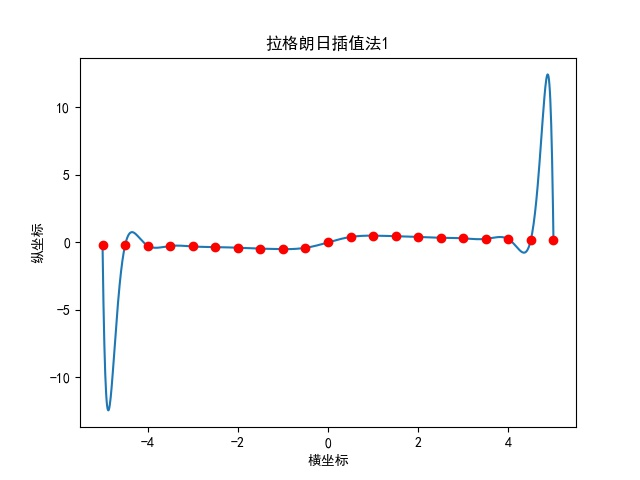
\includegraphics[width=\linewidth]{Lg1.jpg}
    \end{minipage}%
    \begin{minipage}[t]{0.4\linewidth}
    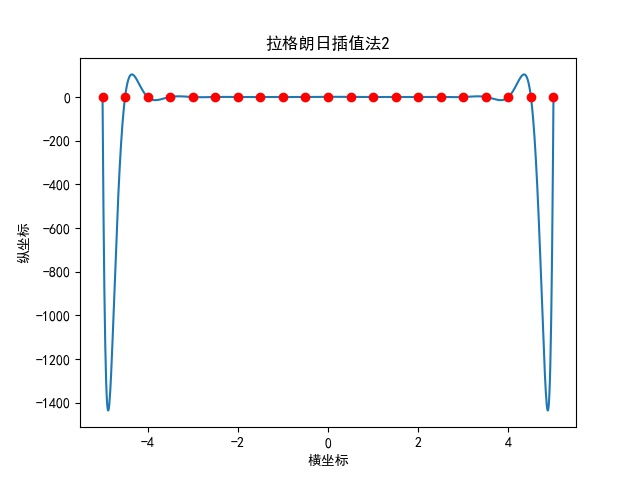
\includegraphics[width=\linewidth]{Lg2.jpg}
    \end{minipage}
\end{figure}

数据1:

$\phi(-3.75) = -0.3856 ,\phi(0.25) = 0.2300$,$R(-3.75)= 0.1367, R(0.25) = 0.0053$.

数据2:

$\phi(-3.75) = -12.6479 ,\phi(0.25) = 0.7044$,$R(-3.75)= 12.6507, R(0.25) = -0.3142$.


\quad

牛顿多项式插值法:
\begin{figure}[h]
    \centering
    \begin{minipage}[t]{0.4\linewidth}
    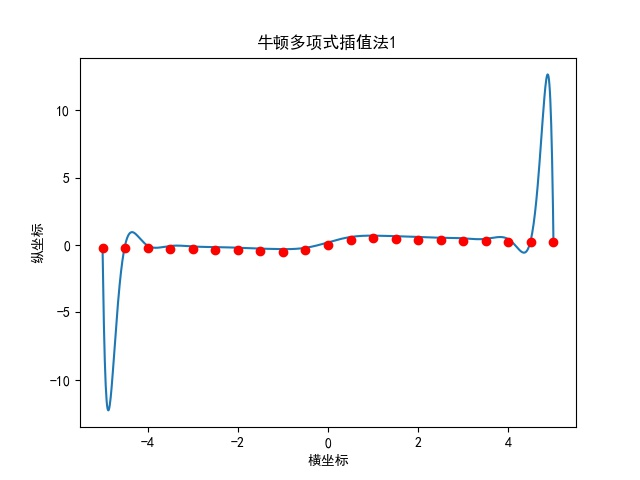
\includegraphics[width=\linewidth]{NT1.jpg}
    \end{minipage}%
    \begin{minipage}[t]{0.4\linewidth}
    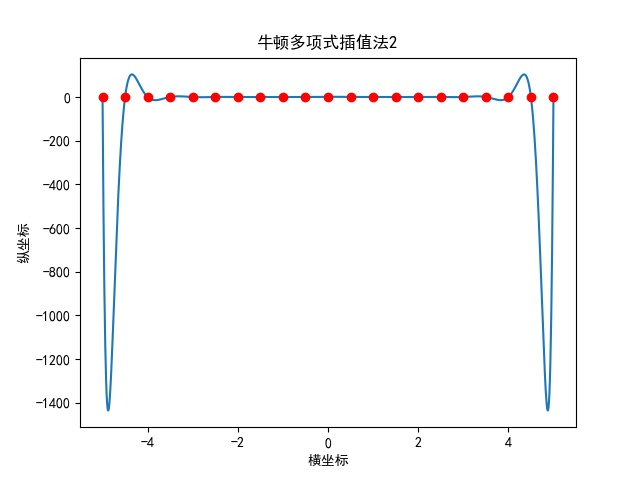
\includegraphics[width=\linewidth]{NT2.jpg}
    \end{minipage}
\end{figure}

数据1:

$\phi(-3.75) = -0.1933 ,\phi(0.25) = 0.4223$,$R(-3.75)= -0.05565, R(0.25) = -0.1870$.

数据2:

$\phi(-3.75) = -12.6495 ,\phi(0.25) = 0.7028$,$R(-3.75)= 12.6523, R(0.25) = -0.3126$.

\quad

分段线性插值法:
\begin{figure}[h]
    \centering
    \begin{minipage}[t]{0.4\linewidth}
    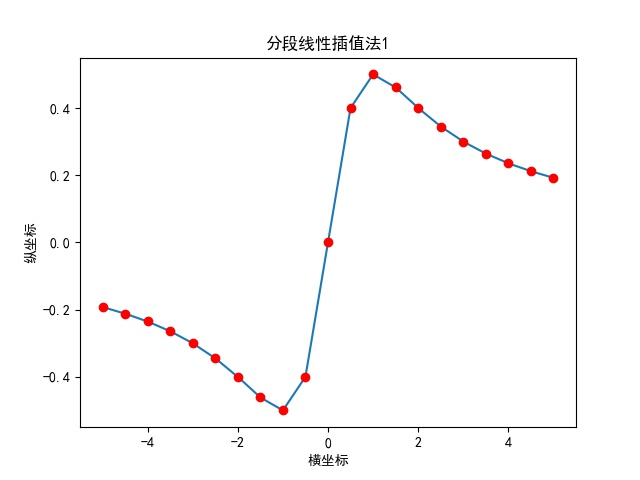
\includegraphics[width=\linewidth]{DL1.jpg}
    \end{minipage}%
    \begin{minipage}[t]{0.4\linewidth}
    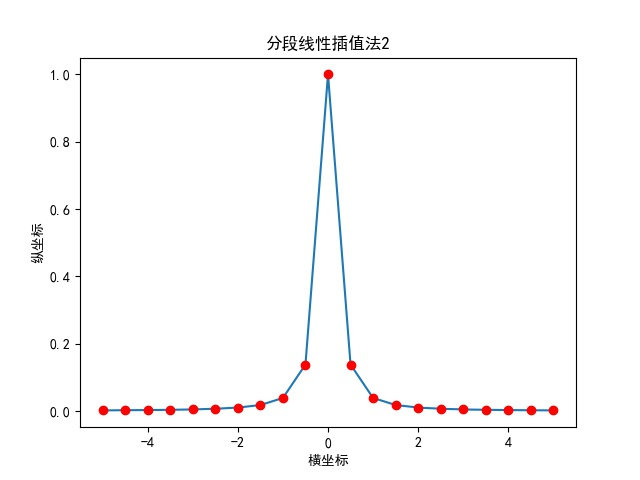
\includegraphics[width=\linewidth]{DL2.jpg}
    \end{minipage}
\end{figure}

数据1:

$\phi(-3.75) = -0.2498 ,\phi(0.25) = 0.2000$,$R(-3.75)= 0.0007873, R(0.25) = 0.03529$.

数据2:

$\phi(-3.75) = 0.0029 ,\phi(0.25) = 0.5690$,$R(-3.75)= -6.3623*10^{-5}, R(0.25) = -0.1787$.

\quad

分析:
结合图像,以及误差分析,显然分段线性插值方法更好。
\subsubsection{附录:源代码}
\begin{lstlisting} [language=python]
  import numpy as np
  from matplotlib import pyplot as plt
  
  plt.rcParams['font.sans-serif'] = ['SimHei']  # 中文字体设置-黑体
  plt.rcParams['axes.unicode_minus'] = False  # 解决保存图像是负号'-'显示为方块的问题
  
  x = np.linspace(-5, 5, 21)
  y1 = [-0.1923, -0.2118, -0.2353, -0.2642, -0.3, -0.3448, -0.4000, -0.4615, -0.5000, -0.4000, 0,
        0.4000, 0.5000, 0.4615, 0.4000, 0.3448, 0.3000, 0.2642, 0.2353, 0.2118, 0.1923]
  y2 = [0.0016, 0.002, 0.0025, 0.0033, 0.0044, 0.0064, 0.0099, 0.0175, 0.0385, 0.1379, 1.0000,
        0.1379, 0.0385, 0.0175, 0.0099, 0.0064, 0.0044, 0.0033, 0.0025, 0.0020, 0.0016]
  find = [-3.75, 0.25]
  
  data1 = []
  for i in range(len(x)):
      data1.append([x[i], y1[i]])
  
  data2 = []
  for i in range(len(x)):
      data2.append([x[i], y2[i]])
  
  
  # 拉格朗日
  def Lg(data, testdata):
      predict = 0
      data_x = [data[i][0] for i in range(len(data))]
      data_y = [data[i][1] for i in range(len(data))]
      if testdata in data_x:
          return data_y[data_x.index(testdata)]
      for i in range(len(data_x)):
          af = 1
          for j in range(len(data_x)):
              if j != i:
                  af *= (1.0 * (testdata - data_x[j]) / (data_x[i] - data_x[j]))
          predict += data_y[i] * af
      return predict
  
  
  def plot_Lg(data, nums, cnt):
      data_x = [data[i][0] for i in range(len(data))]
      data_y = [data[i][1] for i in range(len(data))]
  
      X = np.linspace(min(data_x), max(data_x), nums)
      Y = [Lg(data, x) for x in X]
  
      plt.plot(X, Y, label='result')
      for i in range(len(data_x)):
          plt.plot(data_x[i], data_y[i], 'ro', label='point')
  
      plt.xlabel('横坐标')
      plt.ylabel('纵坐标')
      plt.title('拉格朗日插值法' + str(cnt))
      plt.savefig('Lg' + str(cnt) + '.jpg')
      plt.show()
  
  
  # 分段线性插值
  def DivideLine(data, testdata):
      data_x = [data[i][0] for i in range(len(data))]
      data_y = [data[i][1] for i in range(len(data))]
  
      if testdata in data_x:
          return data_y[data_x.index(testdata)]
      else:
          index = 0
          for j in range(len(data_x)):
              if data_x[j] < testdata < data_x[j + 1]:
                  index = j
                  break
          predict = 1.0 * (testdata - data_x[index]) * \
                    (data_y[index + 1] - data_y[index]) / (data_x[index + 1] - data_x[index]) + data_y[index]
          return predict
  
  
  def plot_DL(data, nums, cnt):
      data_x = [data[i][0] for i in range(len(data))]
      data_y = [data[i][1] for i in range(len(data))]
  
      X = np.linspace(min(data_x), max(data_x), nums)
      Y = [DivideLine(data, x) for x in X]
  
      # print('数据' + str(cnt) + ':')
      # for i in find:
      #     print(i, Y[X.tolist().index(i)])
  
      plt.plot(X, Y, label='result')
  
      for i in range(len(data_x)):
          plt.plot(data_x[i], data_y[i], 'ro', label='point')
  
      plt.xlabel('横坐标')
      plt.ylabel('纵坐标')
      plt.title('分段线性插值法' + str(cnt))
      plt.savefig('DL' + str(cnt) + '.jpg')
      plt.show()
  
  
  # 牛顿插值
  def calF(data):
      data_x = [data[i][0] for i in range(len(data))]
      data_y = [data[i][1] for i in range(len(data))]
  
      F = [1 for _ in range(len(data))]
      FM = []
      for i in range(len(data)):
          FME = []
          if i == 0:
              FME = data_y
          else:
              for j in range(len(FM[len(FM) - 1]) - 1):
                  delta = data_x[i + j] - data_x[j]
                  value = 1.0 * (FM[len(FM) - 1][j + 1] - FM[len(FM) - 1][j]) / delta
                  FME.append(value)
          FM.append(FME)
      F = [fme[0] for fme in FM]
      # print(FM)
      return F
  
  
  def NT(data, testdata, F):
      predict = 0
      data_x = [data[i][0] for i in range(len(data))]
      data_y = [data[i][1] for i in range(len(data))]
      if testdata in data_x:
          return data_y[data_x.index(testdata)]
      else:
          for i in range(len(data_x)):
              Eq = 1
              if i != 0:
                  for j in range(i):
                      Eq = Eq * (testdata - data_x[j])
                  predict += (F[i] * Eq)
      return predict
  
  
  def plot_NT(data, nums, cnt):
      data_x = [data[i][0] for i in range(len(data))]
      data_y = [data[i][1] for i in range(len(data))]
  
      X = np.linspace(min(data_x), max(data_x), nums)
  
      F = calF(data)
      Y = [NT(data, x, F) for x in X]
  
      plt.plot(X, Y, label='result')
      for i in range(len(data_x)):
          plt.plot(data_x[i], data_y[i], 'ro', label='point')
  
      plt.xlabel('横坐标')
      plt.ylabel('纵坐标')
      plt.title('牛顿多项式插值法' + str(cnt))
      plt.savefig('NT' + str(cnt) + '.jpg')
      plt.show()
  
  
  def func1(x):
      return x / (1 + x * x)
  
  
  def func2(x):
      return 1 / (1 + 25 * x * x)
  
  
  plot_Lg(data1, 1000, 1)
  plot_Lg(data2, 1000, 2)
  
  plot_NT(data1, 1000, 1)
  plot_NT(data2, 1000, 2)
  
  plot_DL(data1, 1000, 1)
  plot_DL(data2, 1000, 2)
  
  print('拉格朗日插值法:')
  print('数据1:')
  print(Lg(data1, -3.75), Lg(data1, 0.25))
  print('R(-3.75)=', func1(-3.75) - Lg(data1, -3.75))
  print('R(0.25)=', func1(0.25) - Lg(data1, 0.25))
  
  print('数据2:')
  print(Lg(data2, -3.75), Lg(data2, 0.25))
  print('R(-3.75)=', func2(-3.75) - Lg(data2, -3.75))
  print('R(0.25)=', func2(0.25) - Lg(data2, 0.25))
  
  print()
  
  print('牛顿多项式插值法:')
  F1 = calF(data1)
  F2 = calF(data2)
  print('数据1:')
  print(NT(data1, -3.75, F1), NT(data1, 0.25, F1))
  print('R(-3.75)=', func1(-3.75) - NT(data1, -3.75, F1))
  print('R(0.25)=', func1(0.25) - NT(data1, 0.25, F1))
  
  print('数据2:')
  print(NT(data2, -3.75, F2), NT(data2, 0.25, F2))
  print('R(-3.75)=', func2(-3.75) - NT(data2, -3.75, F2))
  print('R(0.25)=', func2(0.25) - NT(data2, 0.25, F2))
  
  print()
  
  print('分段线性插值法:')
  print('数据1:')
  print(DivideLine(data1, -3.75), DivideLine(data1, 0.25))
  print('R(-3.75)=', func1(-3.75) - DivideLine(data1, -3.75))
  print('R(0.25)=', func1(0.25) - DivideLine(data1, 0.25))
  
  print('数据2:')
  print(DivideLine(data2, -3.75), DivideLine(data2, 0.25))
  print('R(-3.75)=', func2(-3.75) - DivideLine(data2, -3.75))
  print('R(0.25)=', func2(0.25) - DivideLine(data2, 0.25))
  
  print()
  
  for x in find:
      print(x, func1(x), end=' ')
  print()
  for x in find:
      print(x, func2(x), end=' ')    
\end{lstlisting}

\newpage

\section{最小二乘拟合的实验与分析}
\subsection{综合实验:石油产量预测}
\subsubsection{实验题目}
比较不同拟合函数的预测精度。

世界石油产量以每天百万桶计,如下表所示,求最佳最小二乘法数值估计:

$$
\begin{array}{|c|c|c|c|}
    \hline \text { 年 } & \text { 桶/天 }\left(\times 10^{6}\right) & \text { 年 } & \text { 桶/天 }\left(\times 10^{6}\right) \\
    \hline 1994 & 67.052 & 1999 & 72.063 \\
    \hline 1995 & 68.008 & 2000 & 74.669 \\
    \hline 1996 & 69.803 & 2001 & 74.487 \\
    \hline 1997 & 72.024 & 2002 & 74.065 \\
    \hline 1998 & 73.400 & 2003 & 76.777 \\
    \hline
    \end{array}
$$



1.分别分析采用(a)直线,(b)抛物线,(c)立方曲线拟合10个数据点的结果,写出拟合后
的具体函数表达式。

2.进行如表1的残差分析。就残差分析结果
而言,哪一种拟合最好的代表了这些数据? 

3.利用上面的每一种拟合来估计2010年的
石油生产水平,讨论结果。
\subsubsection{算法介绍}
假设 “逼近" 规律的近似函数为 $y=f(x)$, 即有
$$
y_{i}^{*}=f\left(x_{i}\right) \quad i=1,2, \ldots, m
$$

它与观测值 $y_{i}$ 之差 $\delta_{i}=y_{i}^{*}-y_{i}=f\left(x_{i}\right)-y_{i}$ 称为残差。

残差大大小可以作为衡量近似函数好坏的标准。按照
使残差的平方和 $\sum \delta_{i}^{2}$ 最小的规则求得近似函数 $y=f(x)$ 的方
法称为最佳平方逼近, 也称为曲线拟合的最小二乘法。
\subsubsection{实验结果及分析}
\begin{figure}[h]
  \centering
  \begin{minipage}[t]{0.6\linewidth}
  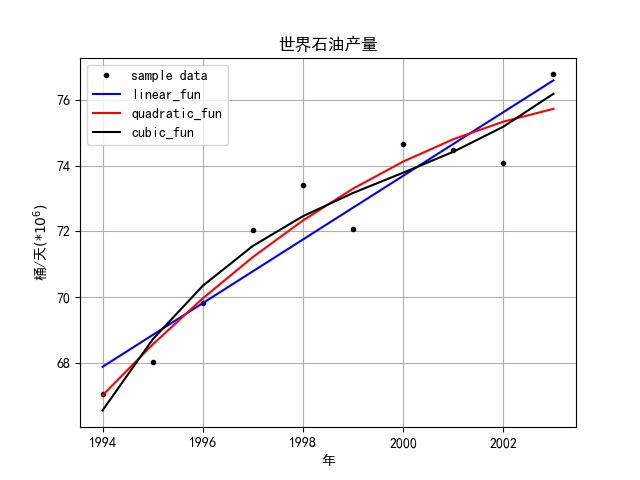
\includegraphics[width=\linewidth]{predict.jpg}
  \end{minipage}
\end{figure}

直线:
$f_1(x) = 0.9693(x-1994) + 67.8727$

抛物线:
$f_2(x) = -0.0723(x-1994)^2 + 1.6203(x-1994) + 67.0048$

立方曲线:
$f_3(x) = 0.0182(x-1994)^3 - 0.3184(x-1994)^2 + 2.4604(x-1994) + 66.5455$

$$
\begin{array}{|c|c|c|c|}
  \hline \text {多项式类型} & \text { 二范数的平方 }& \text { 残差的标准差 } & \text {残差绝对值的均值}\\
  \hline \text {直线} & 9.528 & 0.976 & 0.811 \\
  \hline \text {抛物线} & 6.766 & 0.823 & 0.704 \\
  \hline \text {立方曲线} & 5.740 & 0.758 & 0.691 \\
  \hline
  \end{array}
$$

从数值上看,立方曲线的拟合效果最好。

估计2010年的石油生产水平,$f_1(2010) = 83.382, f_2(2010) = 74.413, f_3(2010) = 99.061$。
从之前的拟合效果来看应当立方曲线的预测值较为准确,为99.061。

\subsubsection{附录:源代码}
\begin{lstlisting} [language=python]
  import math
  import matplotlib.pyplot as plt
  import matplotlib as mpl
  from scipy.optimize import leastsq
  import numpy as np
  
  plt.rcParams['font.sans-serif'] = ['SimHei']  # 中文字体设置-黑体
  plt.rcParams['axes.unicode_minus'] = False  # 解决保存图像是负号'-'显示为方块的问题
  
  x0 = np.arange(1994, 2004, 1, dtype='float')
  x = np.asarray([i-1994 for i in x0])
  y = np.array([67.052, 68.008, 69.803, 72.024, 73.400, 72.063, 74.6669, 74.487, 74.065, 76.777])
  plt.figure()
  plt.title('世界石油产量')
  plt.xlabel('年')
  plt.ylabel('桶/天$(*10^6)$')
  plt.grid(True)
  plt.plot(x0, y, 'k.')
  
  param1 = [0, 0]
  
  
  def linear_fun(s, x):
      k, b = s
      return k * x + b
  
  
  param2 = [0, 0, 0]
  
  
  def quadratic_fun(s, x):
      k1, k2, b = s
      return k1 * x ** 2 + k2 * x + b
  
  
  param3 = [0, 0, 0, 0]
  
  
  def cubic_fun(s, x):
      k1, k2, k3, b = s
      return k1 * x ** 3 + k2 * x ** 2 + k3 * x + b
  
  
  def dist(a, fun, x, y):
      return fun(a, x) - y
  
  
  funs = [linear_fun, quadratic_fun, cubic_fun]
  params = [param1, param2, param3]
  colors = ['blue', 'red', 'black']
  fun_name = ['linear_fun', 'quadratic_fun', 'cubic_fun']
  
  for i, (func, param, color, name) in enumerate(zip(funs, params, colors, fun_name)):
      var = leastsq(dist, param, args=(func, x, y))
      print('[%s] 二范数: %.4f, abs(bias): %.4f, bias_std: %.4f' % (name,
                                                                 ((y-func(var[0], x))**2).sum(),
                                                                 (y-func(var[0], x)).std(),
                                                                 (abs((y-func(var[0], x))).mean())))
      print(var[0])
      print(func(var[0], 2010-1994))
      plt.plot(x0, func(var[0], x), color)
  plt.legend(['sample data', 'linear_fun', 'quadratic_fun', 'cubic_fun'], loc='upper left')
  plt.savefig('predict.jpg')
  plt.show()    
\end{lstlisting}

\newpage

\section{数值积分、微分和常微分方程的数值解法}
\subsection{数值积分}
\subsubsection{题目一}
用梯形公式计算积分$\int_{0}^{1} x^{2} \mathrm{~d} x$。

解:

$$
\int_{0}^{1} x^{2} \mathrm{~d} x = \int_{0}^{1} x\mathrm{~d} x \approx\frac{1-0}{2}[f(1)+f(0)]
=\frac{1}{2}
$$


\subsubsection{题目二}
用辛普森公式计算积分$\int_{1}^{2} \sqrt{x} d x$。

解:
\begin{equation}\nonumber
    \begin{split}
        \int_{1}^{2} \sqrt{x} \mathrm{d} x & \approx \frac{h}{3}\left[f(1)+4 f\left(\frac{1+2}{2}\right)+f(2)\right]
        \\ &= \frac{1}{6}\left[1+2\sqrt{6}+\sqrt{2}\right]
        \\ & \approx 1.219
    \end{split}
\end{equation}
\subsubsection{题目三}
分别用4次、6次牛顿-柯特斯公式计算以下积分并与精确值作比较。
$$
\int_{1}^{2}\left(7 x^{6}-4 x^{3}+1\right) \mathrm{d} x
$$

解:

\ding{172}4次:~~~~~4阶对应系数$\frac{7}{90}, \frac{32}{90}, \frac{12}{90}, \frac{32}{90}, 
\frac{7}{90}$, 对区间[1, 2]四等分
\begin{equation}\nonumber
    \begin{split}
        \int_{1}^{2}\left(7 x^{6}-4 x^{3}+1\right) \mathrm{d} x = (2 - 1) \times (\frac{7}{90}\cdot(7-4+1) & +\frac{32}{90}\cdot(7\cdot{1.25}^6-4\cdot{1.25}^3+1)
        \\&+\frac{12}{90}\cdot(7\cdot{1.5}^6-4\cdot{1.5}^3+1)
        \\&+\frac{7}{90}\cdot(7\cdot{1.75}^6-4\cdot{1.75}^3+1)
        \\&+\frac{7}{90}\cdot(7\cdot{2}^6-4\cdot{2}^3+1))
    \end{split}
\end{equation}

\begin{equation}\nonumber
    \begin{split}
        \\& \approx 0.3111+7.0721+8.9646+64.2214+32.4333
        \\& \approx 113.0026
    \end{split}
\end{equation}

\ding{173}6次:~~~~~6阶对应系数$\frac{41}{840}, \frac{216}{840}, \frac{27}{840}, 
\frac{272}{840}, \frac{27}{840}, \frac{216}{840}, \frac{41}{840}$, 
对区间[1, 2]六等分
\begin{equation}\nonumber
    \begin{split}
        \int_{1}^{2}\left(7 x^{6}-4 x^{3}+1\right) \mathrm{d} x = (2 - 1) \times (\frac{41}{840}\cdot(7\cdot{1}^6-4\cdot{1}^3+1) & +\frac{216}{840}\cdot(7\cdot{(\frac{7}{6})}^6-4\cdot{(\frac{7}{6})}^3+1)
        \\&+\frac{27}{840}\cdot(7\cdot{(\frac{4}{3})}^6-4\cdot{(\frac{4}{3})}^3+1)
        \\&+\frac{272}{840}\cdot(7\cdot{(\frac{3}{2})}^6-4\cdot{(\frac{3}{2})}^3+1)
        \\&+\frac{27}{840}\cdot(7\cdot{(\frac{5}{3})}^6-4\cdot{(\frac{5}{3})}^3+1)
        \\&+\frac{216}{840}\cdot(7\cdot{(\frac{11}{6})}^6-4\cdot{(\frac{11}{6})}^3+1)
        \\&+\frac{41}{840}\cdot(7\cdot{2}^6-4\cdot{2}^3+1))
        \\ \approx 112.9997
    \end{split}
\end{equation}

\ding{174}精确解:
\begin{equation}\nonumber
    \begin{split}
        \int_{1}^{2}\left(7 x^{6}-4 x^{3}+1\right) \mathrm{d} x = (x^7-x^4+x){|}^{2}_{1} = 113
    \end{split}
\end{equation}

经过对比,六次牛顿-柯特斯公式更加精确。
\subsection{数值微分}
\subsubsection{题目一}
用三点插值微分公式求各点的一阶和二阶导数,函数$f(x)$由下表给出

$$
\begin{array}{c|c|c|c}
  \hline x_{i} & 1.0 & 1.1 & 1.2 \\
  \hline f\left(x_{i}\right) & 0.2500 & 0.2268 & 0.2066 \\
  \hline
  \end{array}
$$
解:
\begin{equation}\nonumber
    \begin{split}
        f^{'}(x_0) &\approx \frac{1}{2h}\cdot[-3f(x_0)+4f(x_1)-f(x_2)]\\
        &=\frac{1}{0.2} \times (-3\times0.25+4\times0.2268-0.2066)\\
        &= -0.247
    \end{split}
\end{equation}

\begin{equation}\nonumber
    \begin{split}
        f^{'}(x_1) \approx \frac{1}{2h}\cdot[-f(x_0)+f(x_2)]
        &=\frac{1}{0.2} \times (-0.25+0.2066)\\
        &= -0.217
    \end{split}
\end{equation}

\begin{equation}\nonumber
    \begin{split}
        f^{'}(x_2) &\approx \frac{1}{2h}\cdot[f(x_0)-4f(x_1)+3f(x_2)]\\
        &=\frac{1}{0.2} \times (0.25-4\times0.2268+3\times0.2066)\\
        &= -0.187
    \end{split}
\end{equation}

\begin{equation}\nonumber
    \begin{split}
        f^{''}(x_0) &\approx \frac{1}{h^2}\cdot[f(x_0)-2f(x_1)+f(x_2)]\\
        &=\frac{1}{{0.1}^2} \times (0.25-2\times0.2268+0.2066)\\
        &= 0.3
    \end{split}
\end{equation}

\begin{equation}\nonumber
    \begin{split}
        f^{''}(x_1) &\approx \frac{1}{h^2}\cdot[f(x_0)-2f(x_1)+f(x_2)]\\
        &=\frac{1}{{0.1}^2} \times (0.25-2\times0.2268+0.2066)\\
        &= 0.3
    \end{split}
\end{equation}

\begin{equation}\nonumber
    \begin{split}
        f^{''}(x_2) &\approx \frac{1}{h^2}\cdot[f(x_0)-2f(x_1)+f(x_2)]\\
        &=\frac{1}{{0.1}^2} \times (0.25-2\times0.2268+0.2066)\\
        &= 0.3
    \end{split}
\end{equation}

\subsection{常微分方程的数值解法}
\subsubsection{题目一}
分别用欧拉方法、改进欧拉法求解初值问题
$$
y^{\prime}=\frac{t-y}{2}, \quad y(0)=1
$$
在区间[0, 3]上的数值解,取步长为$h=0.5$,比较它们与准确解的误差(已知该初值问题的解析解为
$y(t)=3 e^{-t / 2}-2+t$)。

解:

\ding{172}欧拉方法:

\begin{equation}\nonumber
    \left\{\begin{array}{l}
        y(0)=1 \\
        y_{i+1}=y_{i}+h \cdot \frac{t-y}{2}
        \end{array}\right.
\end{equation}

故:

\begin{longtable}{c|c|c}
    \caption{欧拉方法}\\
    \hline $t_k$ & $y_k$ & $y_{t_k}$\\
    \hline0   & 1.0      & 1\\
     0.5 & 0.75     & 0.836405\\
     1   & 0.6875   & 0.819592\\
     1.5 & 0.765625 & 0.917100\\
     2   & 0.949219 & 1.103638\\
     2.5 & 1.211914 & 1.359514\\
     3   & 1.533936 & 1.669390\\
    \hline      
\end{longtable}


\ding{172}改进欧拉方法:

\begin{equation}\nonumber
    \left\{\begin{array}{c}
        y(0)=1 \\
        y_{i+1}=\frac{4-h}{2 h+4} y_{i}+\frac{h}{2 h+4}\left(t_{i}+t_{i+1}\right)
        \end{array}\right.
\end{equation}

故:

\begin{longtable}{c|c|c}
    \caption{改进欧拉方法}\\
    \hline $t_k$ & $y_k$ & $y_{t_k}$\\
    \hline
    0   & 1.0      & 1\\
     0.5 & 0.85     & 0.836402\\
     1   & 0.845   & 0.819592\\
     1.5 & 0.9415 & 0.917100\\
     2   & 1.10905 & 1.103638\\
     2.5 & 1.326335 & 1.359514\\
     3   & 1.5784345 & 1.669390\\
    \hline      
\end{longtable}
\newpage

\section{总结与心得体会}
\subsection{总结}
我们这门课学习了计算误差、非线性方程求根、线性方程组的解法、矩阵的特征值与特征向量、插值
、拟合与最小二乘法、数值积分与数值微分。

\subsection{心得体会}
这门课程是一个十分重视算法和原理的学科,同时它能够将人的思维引入数学思考的模式,
在处理问题的时候,可以合理适当的提出方案和假设。他的内容贴近实际,像数值分析,数值微分,求解线性方程组的
解等,使数学理论更加有实际意义。

在课后,我们使用计算机编程实践这些算法,让我们对这些算法更加深刻理解,也培养了我们数值分析核心素养,用有穷取代无穷,变不可解
为可解,变不可编程为可编程的方法,对数学问题近似求解,逐步求精。
\end{document}
